\section{nDVCS at CLAS12: kinematics and acceptances}
In order to study the kinematics of the reaction and determine the expected count rates for both the nDVCS signal and its main background ($ed\to en\pi^0(p)$), an event generator for DVCS/BH and exclusive $\pi^0$ electroproduction on the neutron inside a deuterium target has been developed \cite{ahmed}. The DVCS amplitude is calculated according to the BKM formalism \cite{belitski}, where the GPDs have been taken from the standard CLAS DVCS generator \cite{harut}. The Fermi-motion distribution is calculated with the Paris potential \cite{paris}. The exclusive $\pi^0$ electroproduction channel is generated assuming longitudinal dominance within the naive quark model approximation \cite{ahmed}. Note that no smearing effects due to the nuclear ND$_3$ target are included in the event generator. 

The output of the event generator was fed through CLAS12 FASTMC, to simulate the acceptance and resolutions of electrons and photons in the Forward Detector. 

The expected resolutions and acceptance of the CND for neutrons, outlined in the previous sections, were also included in the FastMC code. 

\begin{figure}[t]
\begin{center}
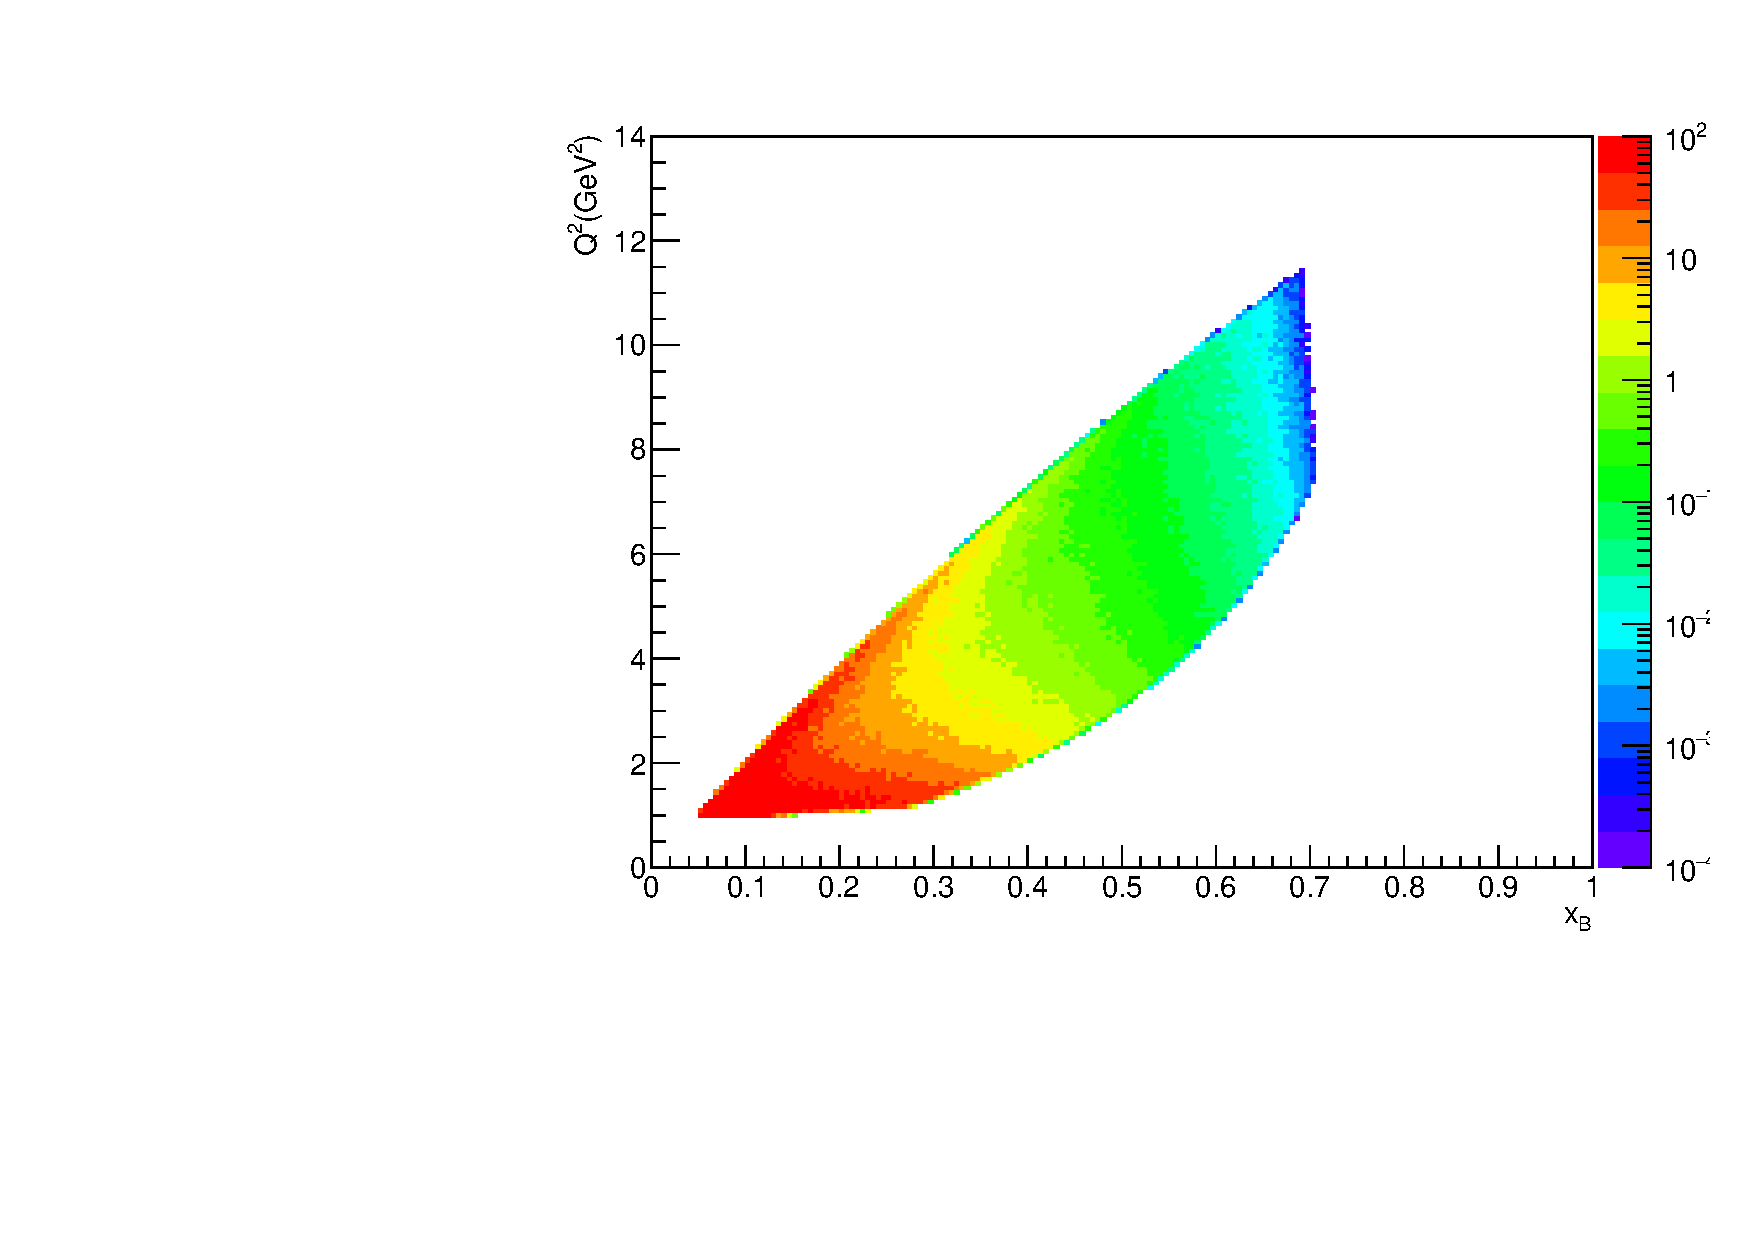
\includegraphics[width=2.9in]{q2vsxb_FT.pdf}
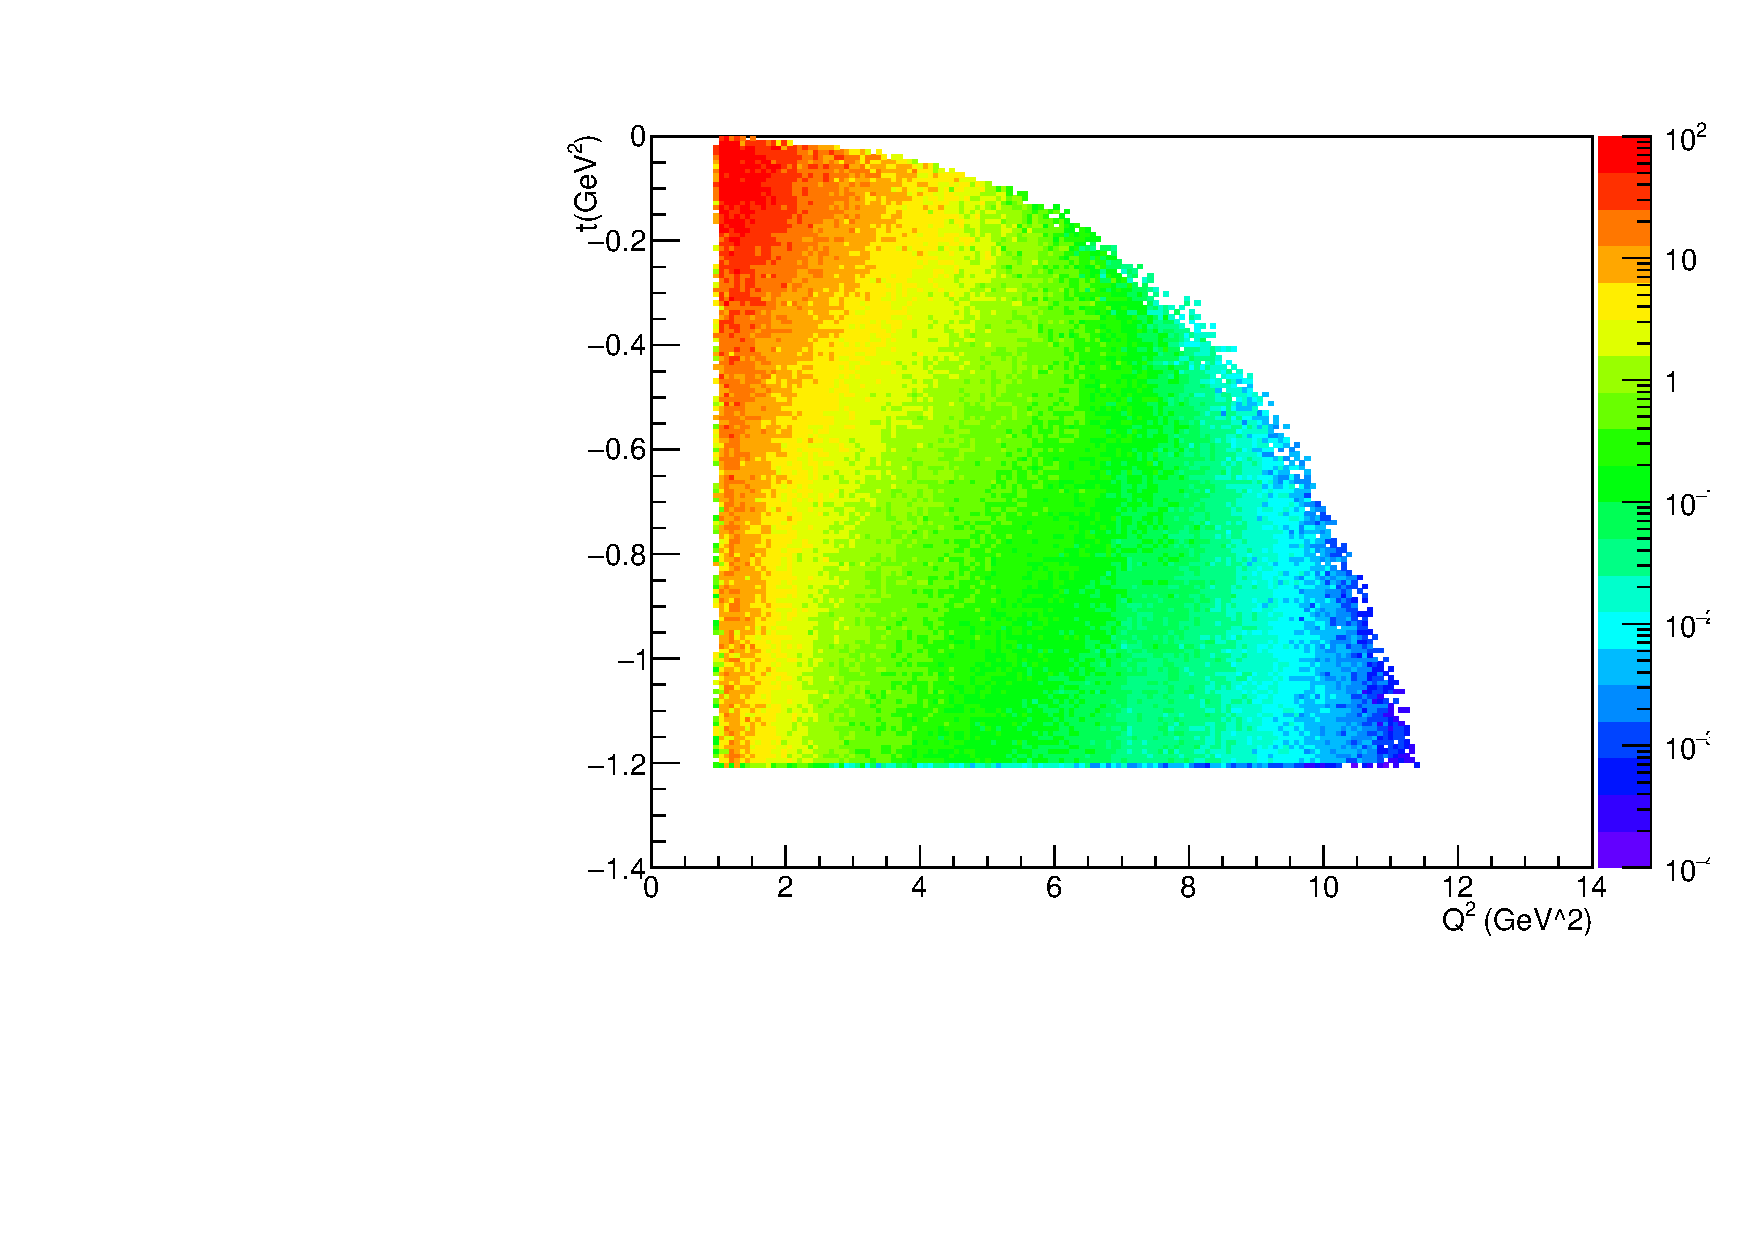
\includegraphics[width=2.9in]{tvsq2_FT.pdf}
\caption [Distributions of kinematic variables for nDVCS events]
{Distributions of kinematic variables for nDVCS events. CLAS12 acceptance cuts and physics cuts are included. Left: $Q^2$ as a function of $x_B$. Right: $t$ as a function of $Q^2$.}
\label{kine_vars}
\end{center}
\end{figure}
Kinematic cuts to ensure the applicability of the GPD formalism ($Q^2>1$ GeV$^2$/c$^2$, $t>-1.2$ GeV$^2$/c$^2$, $W>2$ GeV/c$^2$) have been applied. Figure~\ref{kine_vars} shows the coverage in $Q^2$, $x_B$ and $t$ that is obtained from the event generator for the nDVCS/BH reaction, with an electron-beam energy of 11 GeV. 

 Figures~\ref{e_th_p},~\ref{g_th_p}, and~\ref{n_th_p} show the momentum $p$ as a function of $\theta$ in the lab frame for, respectively, the electron, the photon and the neutron. As expected, the electron and the photon are mostly emitted at forward angles, while the neutron recoils at backwards angles. 

\begin{figure}[bht]
\begin{center}
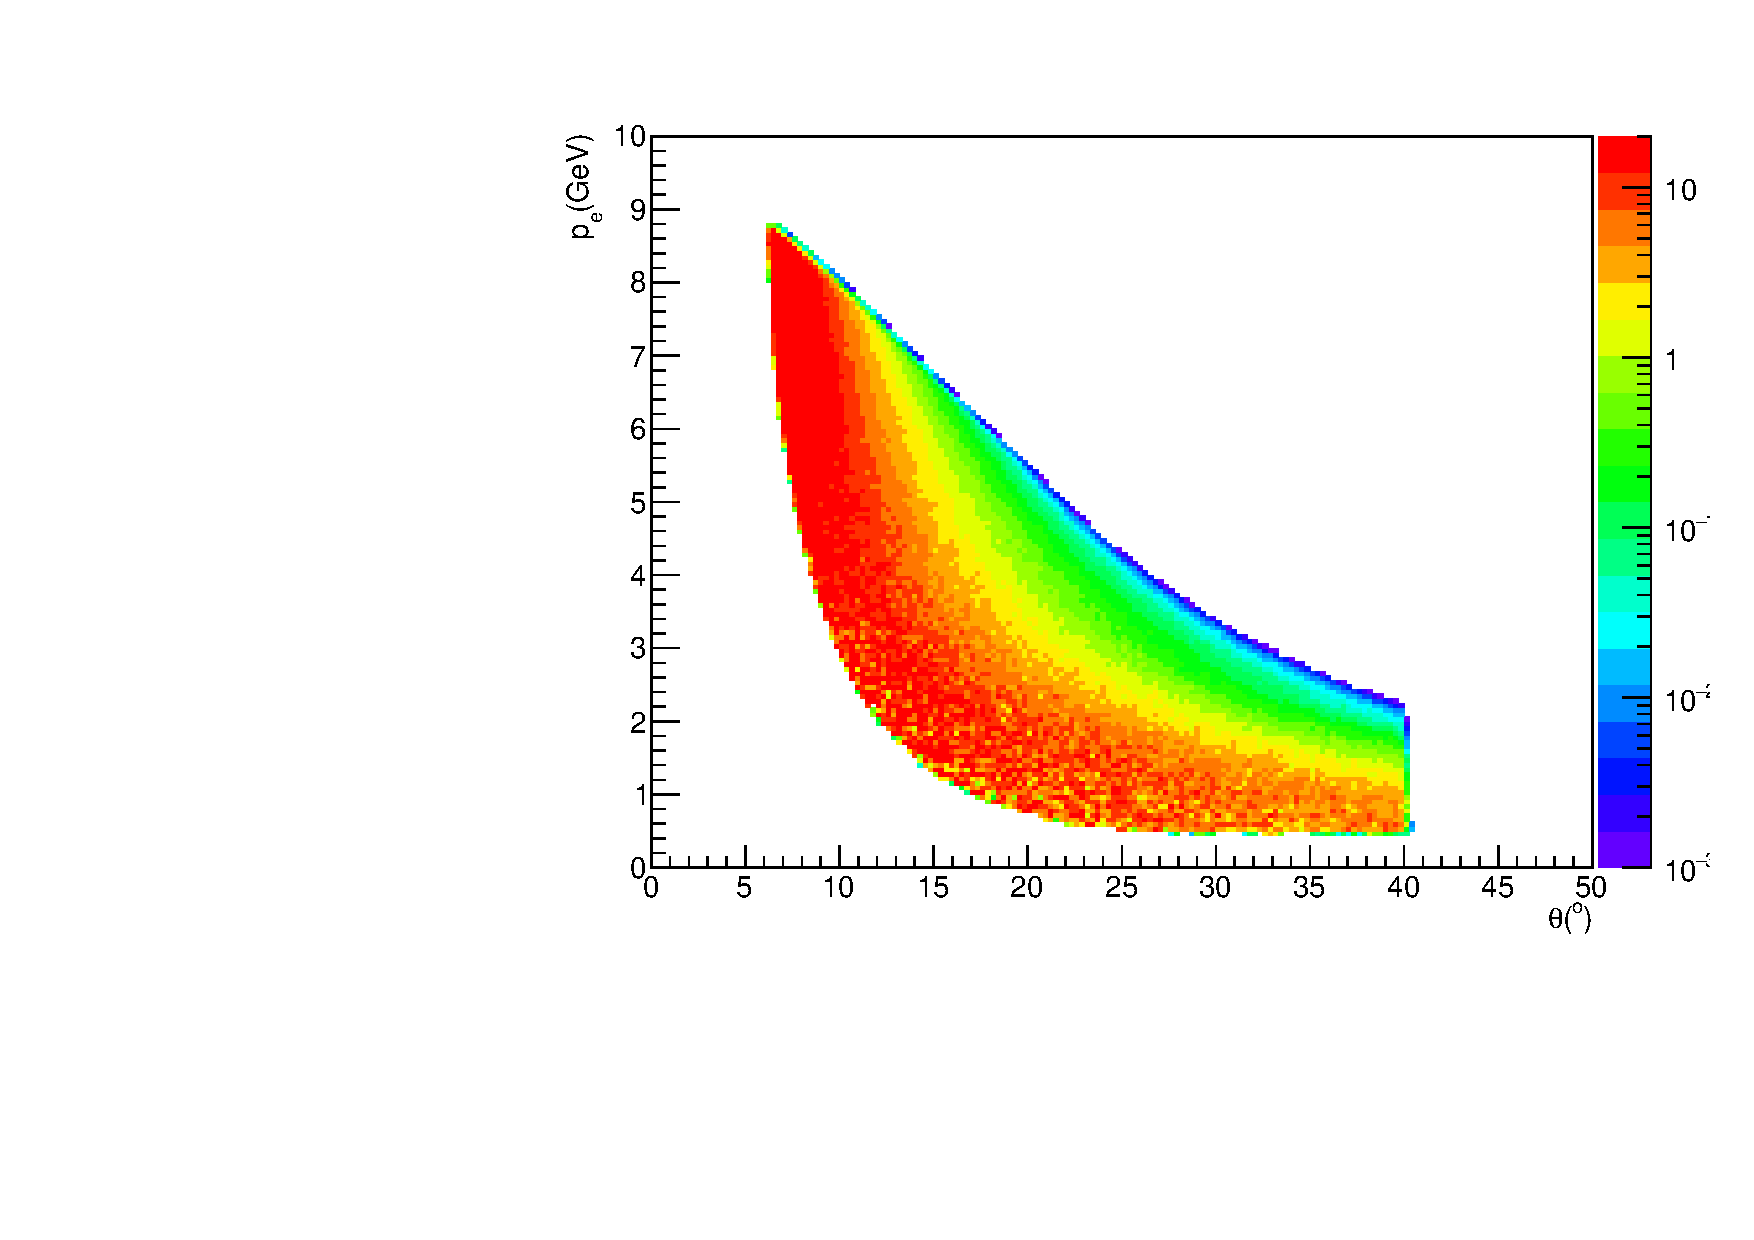
\includegraphics[width=3.2in]{theta_p_el.pdf}
\caption [Electron momentum as a function of electron polar angle]
{Electron momentum as a function of electron polar angle, for nDVCS events. CLAS12 acceptance cuts and physics cuts are included.}
\label{e_th_p}
\end{center}
\end{figure}

\begin{figure}  
\begin{center}
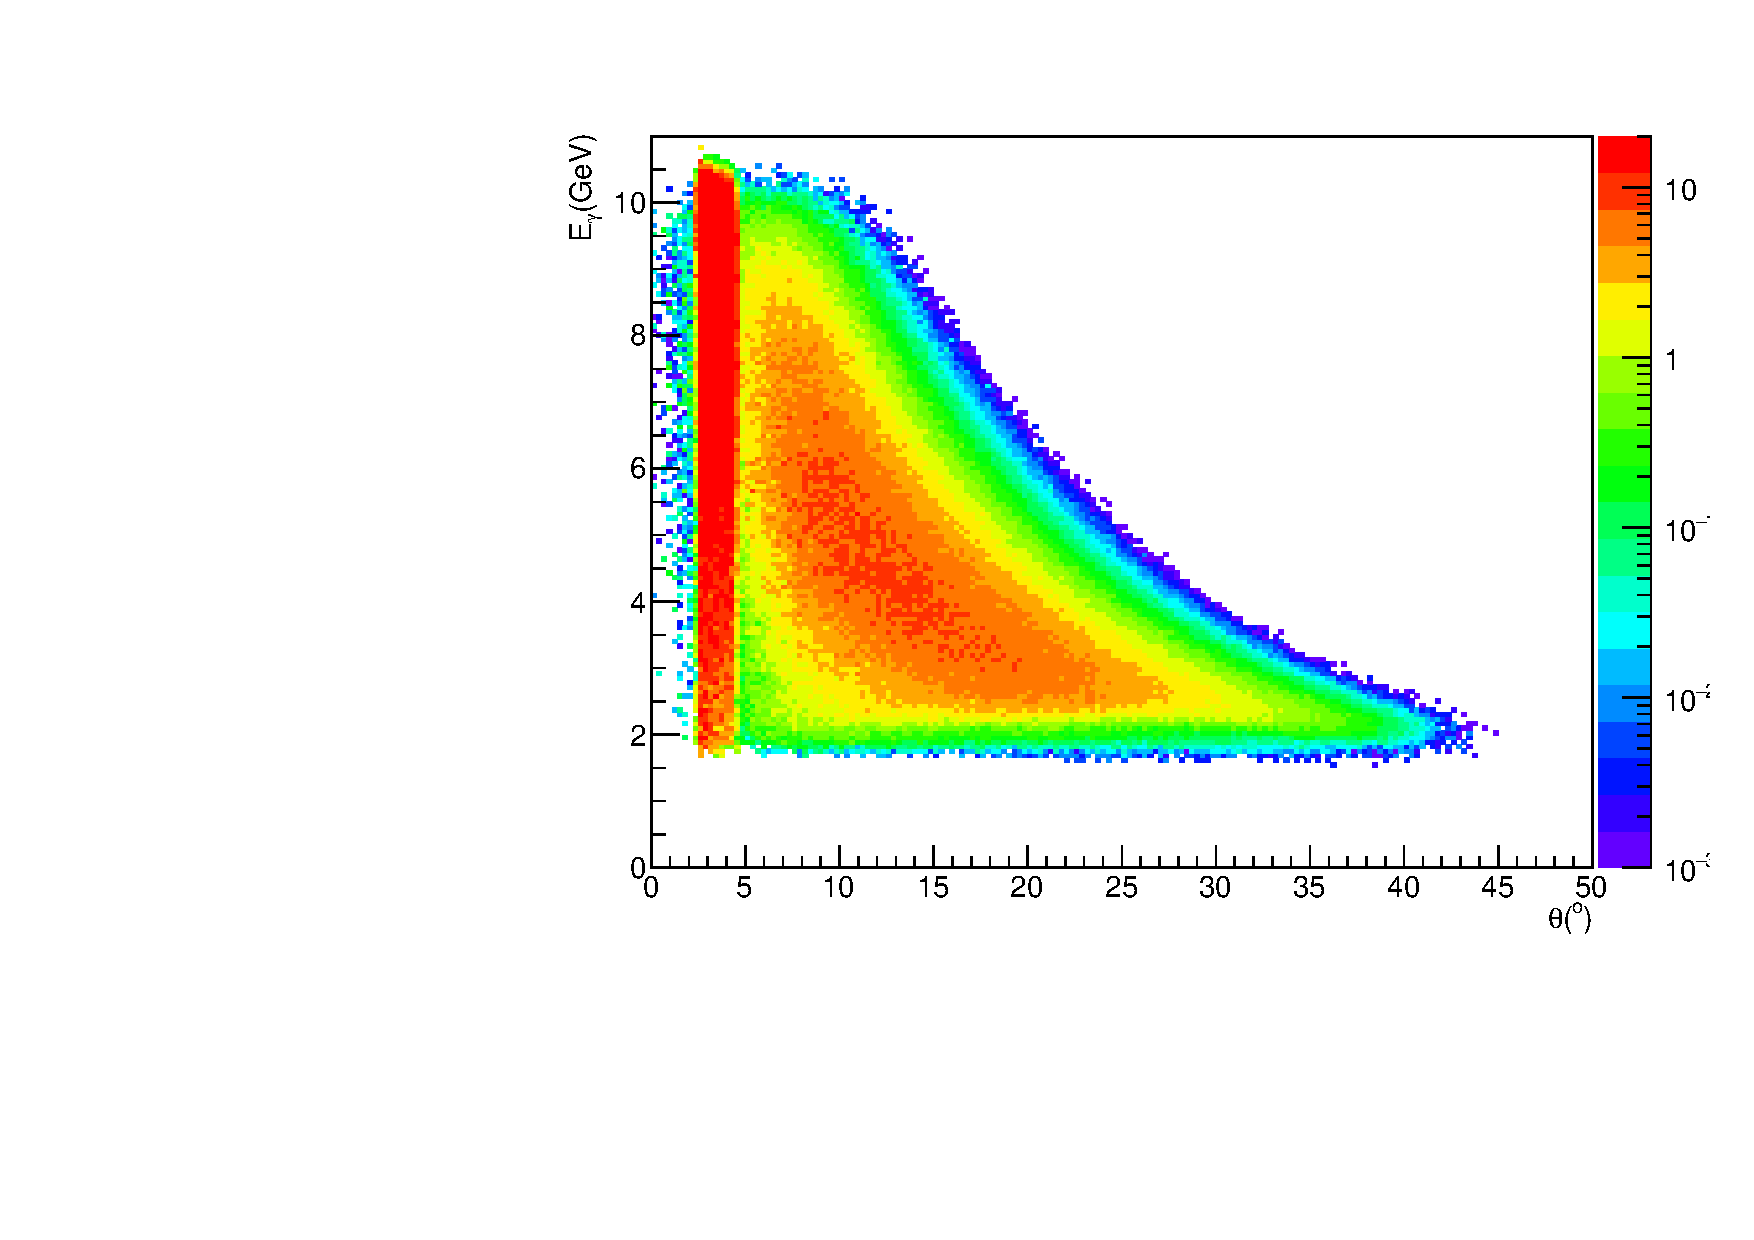
\includegraphics[width=3.2in]{theta_p_phot_FT.pdf}
\caption [Photon momentum as a function of photon polar angle, for nDVCS events]
{Photon momentum as a function of photon polar angle, for nDVCS events. CLAS12 acceptance cuts and physics cuts are included. The vertical band at low $\theta$ corresponds to photons detected in the Forward Tagger.} 
\label{g_th_p}
\end{center}
\end{figure}

\begin{figure}  
\begin{center}
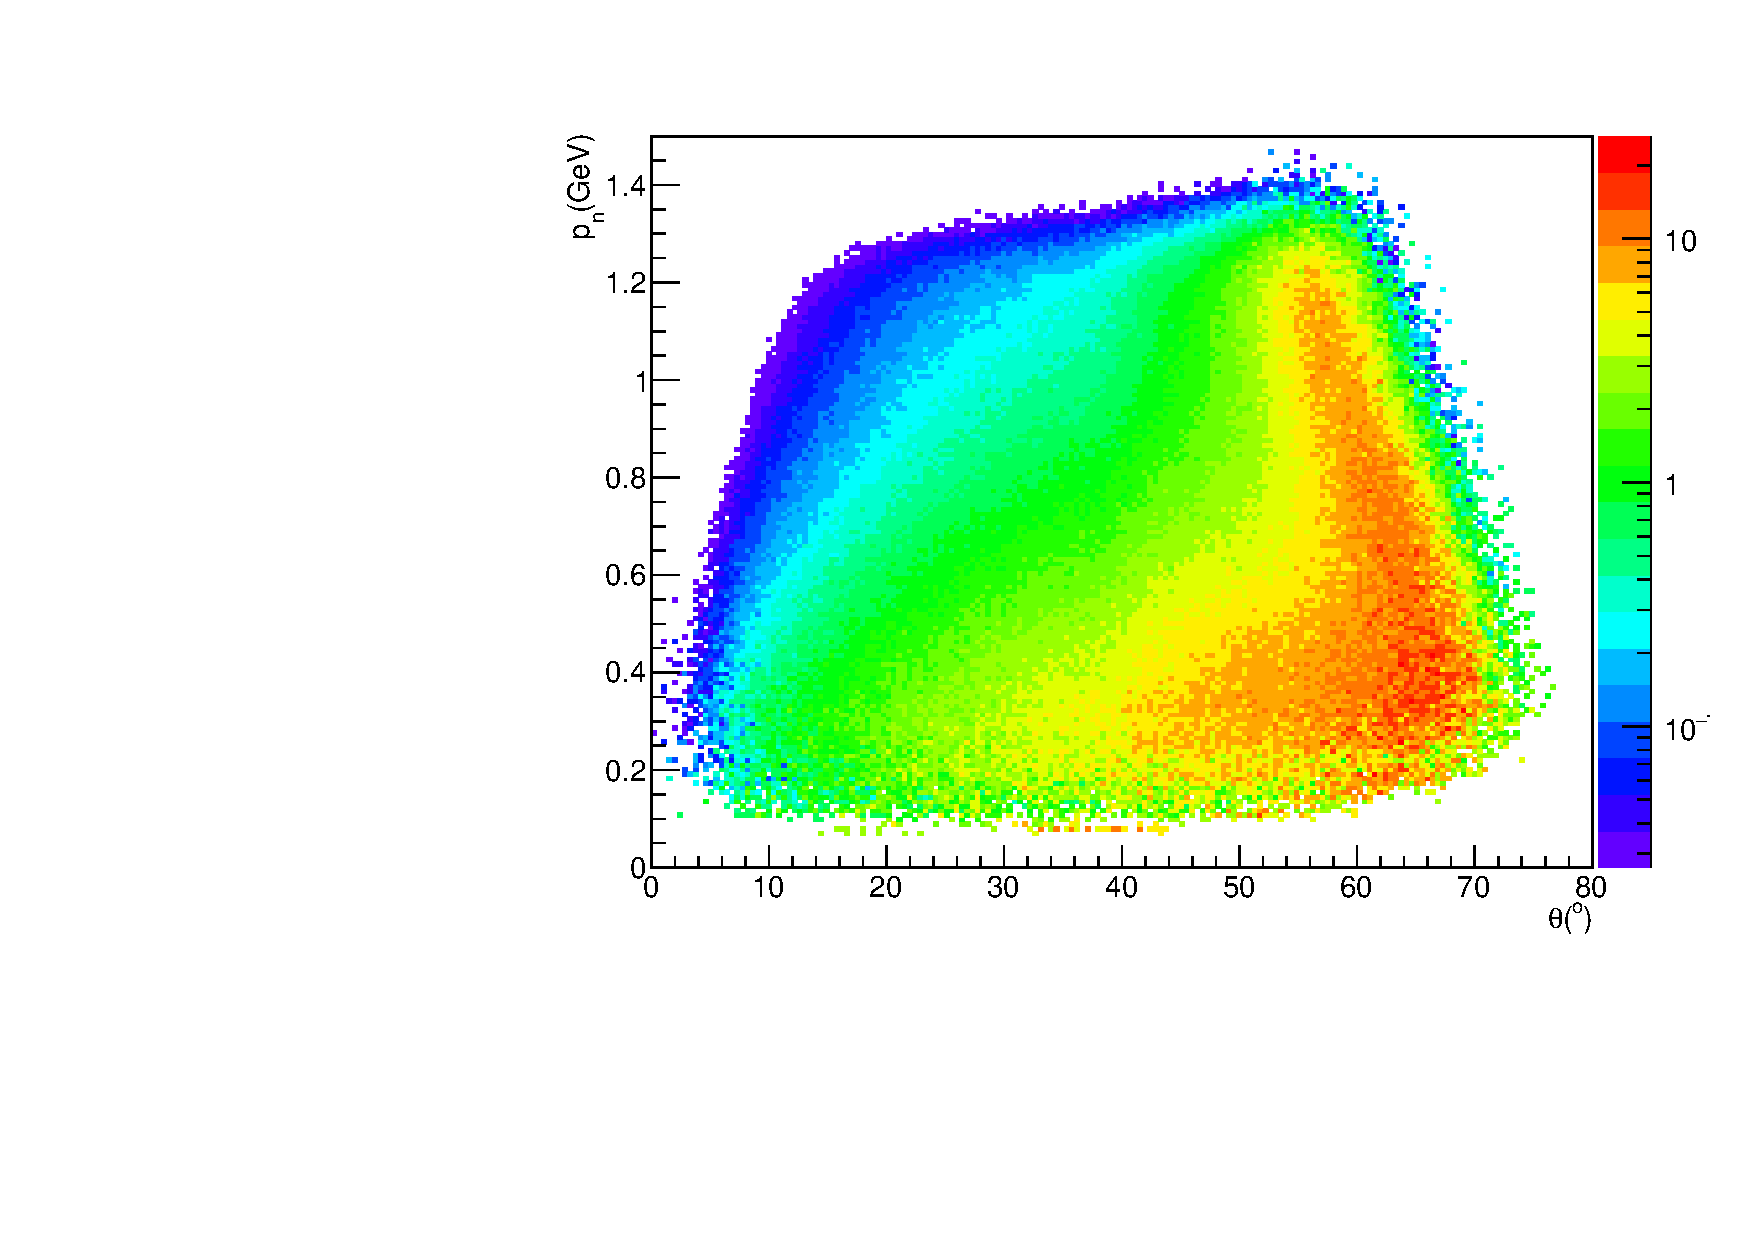
\includegraphics[width=3.2in]{theta_p_neut.pdf}
\caption [Neutron momentum as a function of neutron polar angle]
{Neutron momentum as a function of neutron polar angle, for nDVCS events. CLAS12 acceptance cuts and physics cuts are included.}
\label{n_th_p}
\end{center}
\end{figure}

\section{Measurement of the asymmetries}
We plan to extract two kinds of asymmetries, the experimental definitions of which are given here. In all of the formulae below, the first sign in the superscript on the number of normalized DVCS/BH events $N$ is the beam helicity ($b$) and the second sign
is the target polarization ($t$).
$N$ is obtained from $en\gamma$ events ($N_{en\gamma}$), normalized by the corresponding Faraday-cup charge ($FC^{bt}$) after subtraction of the $\pi^0$ background as follows:
\begin{equation}
N^{bt}= (1-B_{\pi^0}^{bt})\cdot \frac{N^{bt}_{en\gamma}}{FC^{bt}},
\end{equation}

where $B_{\pi^0}$ is the relative $\pi^0$ contamination, outlined in Section \ref{sec_pi0_back}. 

The target-spin asymmetry will be computed as:
\begin{equation}\label{def_tsa}
A_{\rm UL} = \frac{N^{++}+N^{-+}-N^{+-}-N^{--}}{D_f (P_t^-(N^{++}+N^{-+})+P_t^+(N^{+-}+N^{--}))}~.
\end{equation}
 $D_f$ is the dilution factor to account for the contribution of the unpolarized background (Section \ref{sec_dilution}), and $P_t$ is the polarization of the target. 

The double (beam-target) spin asymmetry will be obtained as:

\begin{equation}\label{def_dsa}
A_{\rm LL} = \frac{N^{++}+N^{--}-N^{+-}-N^{-+}}{P_b\cdot D_f (P_t^-(N^{++}+N^{-+})+P_t^+(N^{+-}+N^{--}))}
\end{equation}
where $P_b$ is the polarization of the beam.

In the following, the steps leading to the extraction from the data of all the terms composing these asymmetries will be presented. 

\subsection{Event selection and exclusivity cuts}\label{sec_excl_cuts}
After selecting events with exactly one electron (in the forward part of CLAS12) and one neutron (in the CND and in the EC), and at least one photon (in the EC or in the FT), and applying the appropriate PID and fiducial cuts, further cuts need to be applied to ensure the exclusivity of the DVCS/Bethe-Heitler final state. Two kinds of backgrounds need, in fact, to be removed, or reduced as much as possible: the nuclear background coming from scattering on the nitrogen of the ND$_3$ target, and the background coming from other channels containing electron, neutron and at least one photon in the final state. Having measured the four-vectors of the three active final-state particles, one can construct several observables (hereafter referred to as ``exclusivity variables'') on which cuts can be applied to select the DVCS/BH channel. Here, the following quantities were studied, with the aid of our nDVCS and $en\pi^0(p)$ simulations:
\begin{itemize}
\item{the squared missing mass of $X$, in the $ed\to en\gamma X$ reaction;}
\item{the momentum of the spectator proton, obtained as $p(X)$ from $ed\to en\gamma X$;}
\item{the squared missing mass of $X$, in the $en\to en\gamma X$ reaction, assuming the initial neutron to be at rest;}
\item{the missing energy of $X$, in the $ed\to en\gamma X$ reaction;}
\item{$p_{perp}$, the transverse component of the missing momentum of the reaction $en\to en\gamma X$, given by $p_{perp}=\sqrt{p_x(X)^2+p_y(X)^2}$.}
\end{itemize}

Figures~\ref{dvcs_excl} and \ref{pi0_excl} show the exclusivity variables listed above for, respectively, nDVCS simulated events and $en\pi^0(p)$ simulated events for which only one electron, one neutron and one photon of energy above 2 GeV fell within the CLAS12 acceptance. The red lines represent the exclusivity cuts, the values of which were choosen to maximize the number of nDVCS events retained while reducing the $en\pi^0(p)$ background as much as possible. It must be stressed that the event generator adopted here does not contain Fermi motion effects coming from the nitrogen of the ND$_3$ target. The experimental distributions of the exclusivity variables will therefore be broader, and the peaks will be masked by the nuclear background. 
However, it was shown in the eg1-DVCS analysis \cite{pisano} that peaks due to the pDVCS channel became evident when appropriately rescaled spectra from a $^{12}$C background target were subtracted from the exclusivity variable distributions.  We plan to adopt a similar approach here.

\begin{figure}
\begin{center}
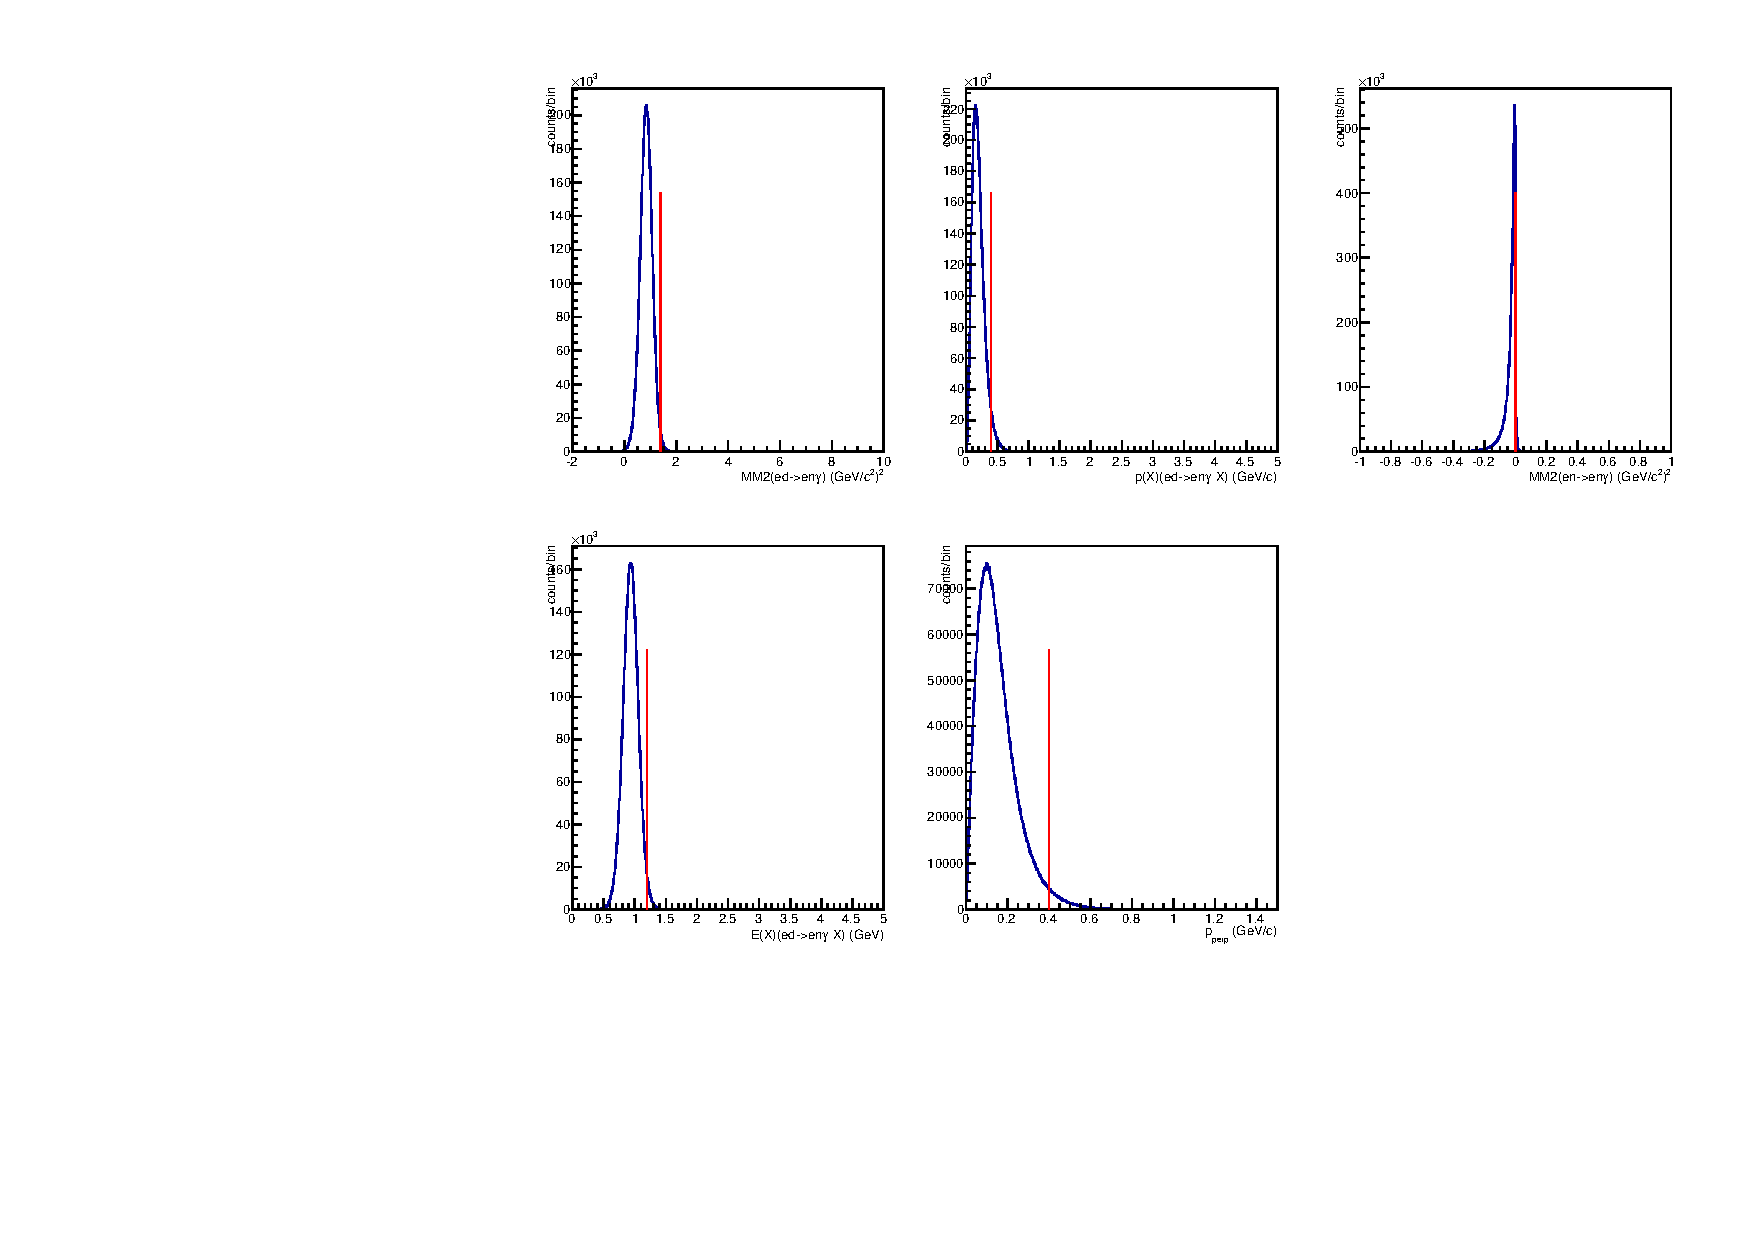
\includegraphics[width=120mm]{dvcs_excl_vars_noFT_100days.pdf}
\caption[nDVCS simulation, after FastMC]
{nDVCS simulation, after FastMC: DVCS exclusivity variables. Starting from the top left: MM$^2_X(ed\to en\gamma X)$, $p(X)(ed\to en\gamma X)$,  MM$^2_X(en\to en\gamma X)$, $E(X)(ed\to en\gamma X)$, $p_{perp}$. The red lines mark the values adopted for the nDVCS exclusivity cuts.}
\label{dvcs_excl}
\end{center}
\end{figure}

\begin{figure}
\begin{center}
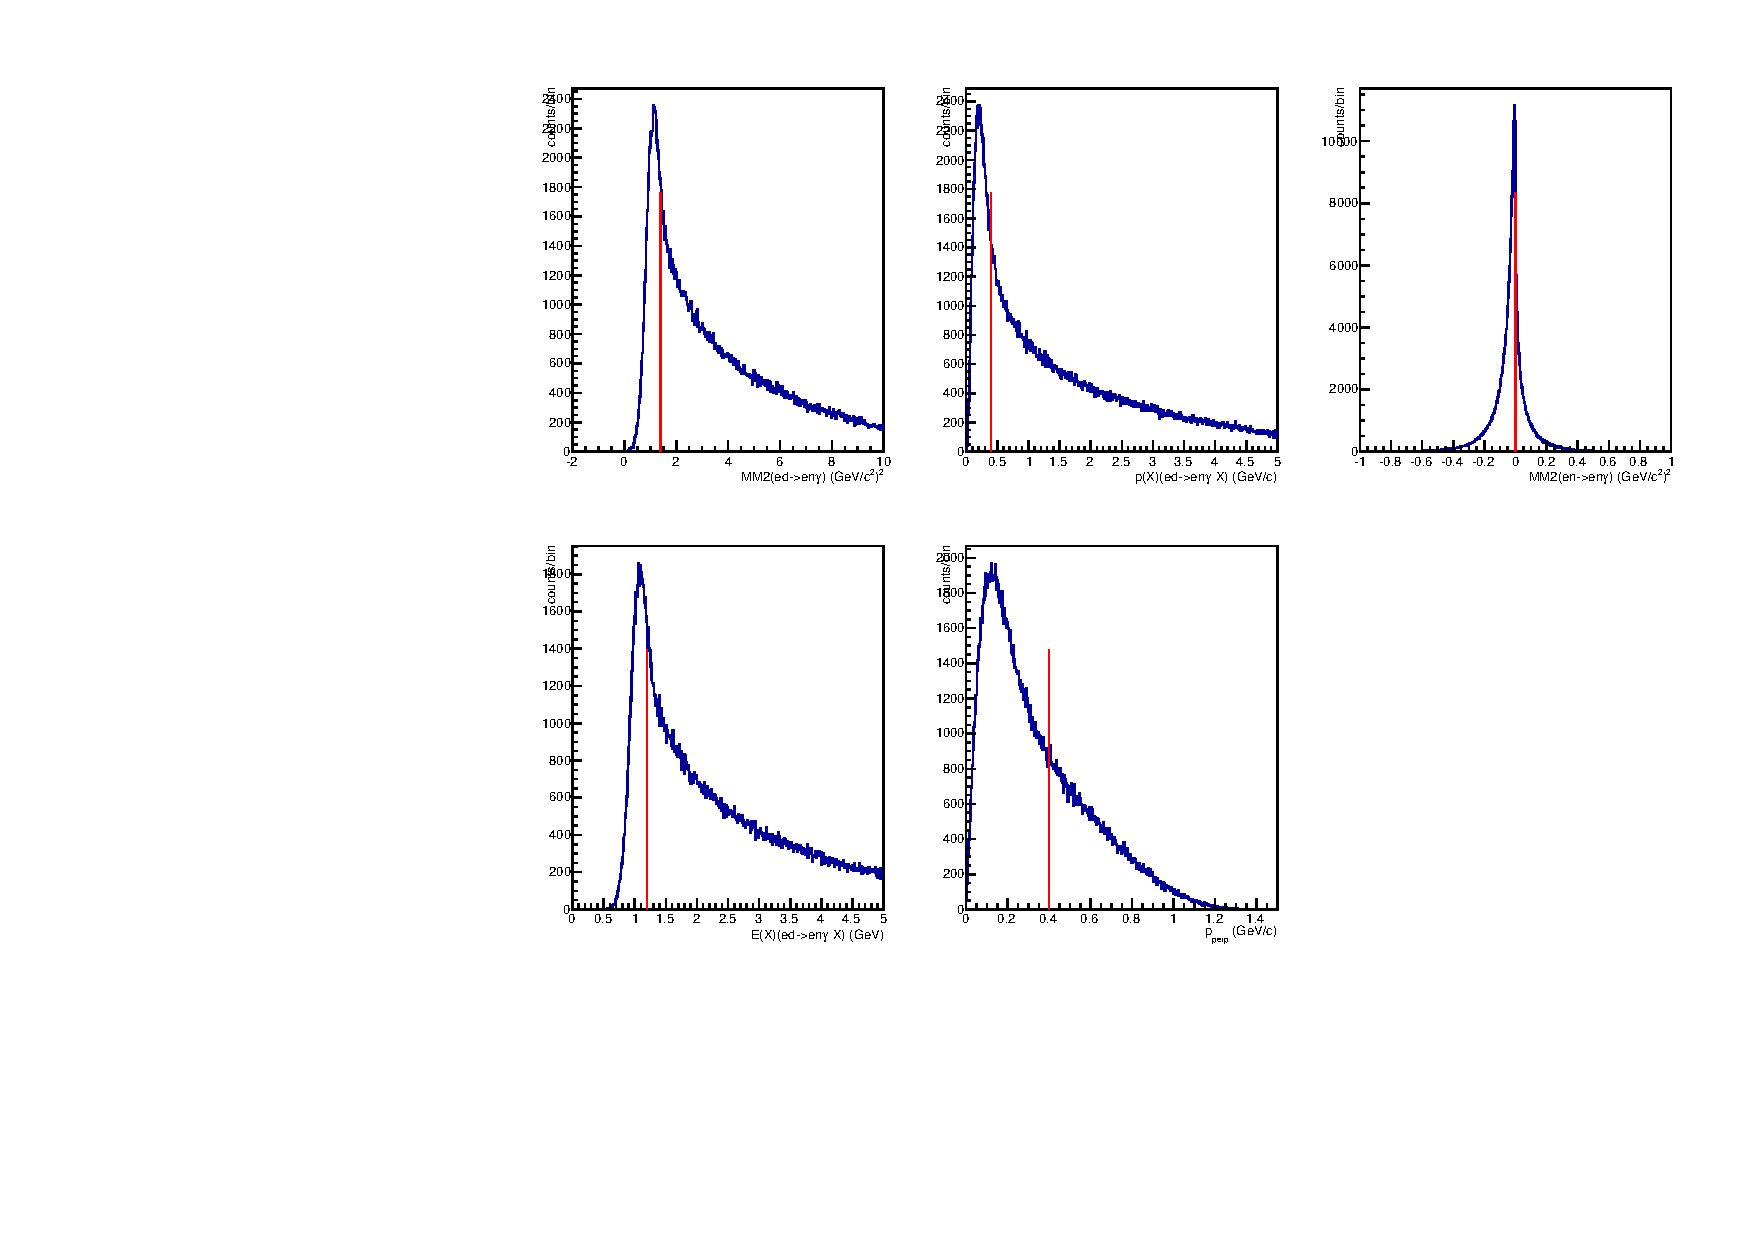
\includegraphics[width=120mm]{pi0_excl_vars_noFT_100days.pdf}
\caption[$\pi^0$ simulation, after FastMC]
{$\pi^0$ simulation, after FastMC, events for which only one electron, one neutron and one photon of energy above 2 GeV fell within the CLAS12 acceptance: DVCS exclusivity variables, same as Fig.~\ref{dvcs_excl}. The red lines mark the values adopted for the nDVCS exclusivity cuts.}
\label{pi0_excl}
\end{center}
\end{figure}

The expected $en\pi^0(p)$ contamination that remains after these cuts is shown in Fig.~\ref{ndvcs-pi0}, where the ratio of surviving $en\pi^0(p)$ events to the number of nDVCS events is plotted as a function of $\phi$, integrated over the other kinematic variables. It ranges from 0, at the extreme $\phi$ values, to about $40\%$, in the central $\phi$ range. This background can be evaluated and subtracted from the final asimmetries, as will be described in Section~\ref{sec_pi0_back}. 

\begin{figure}  
\begin{center}
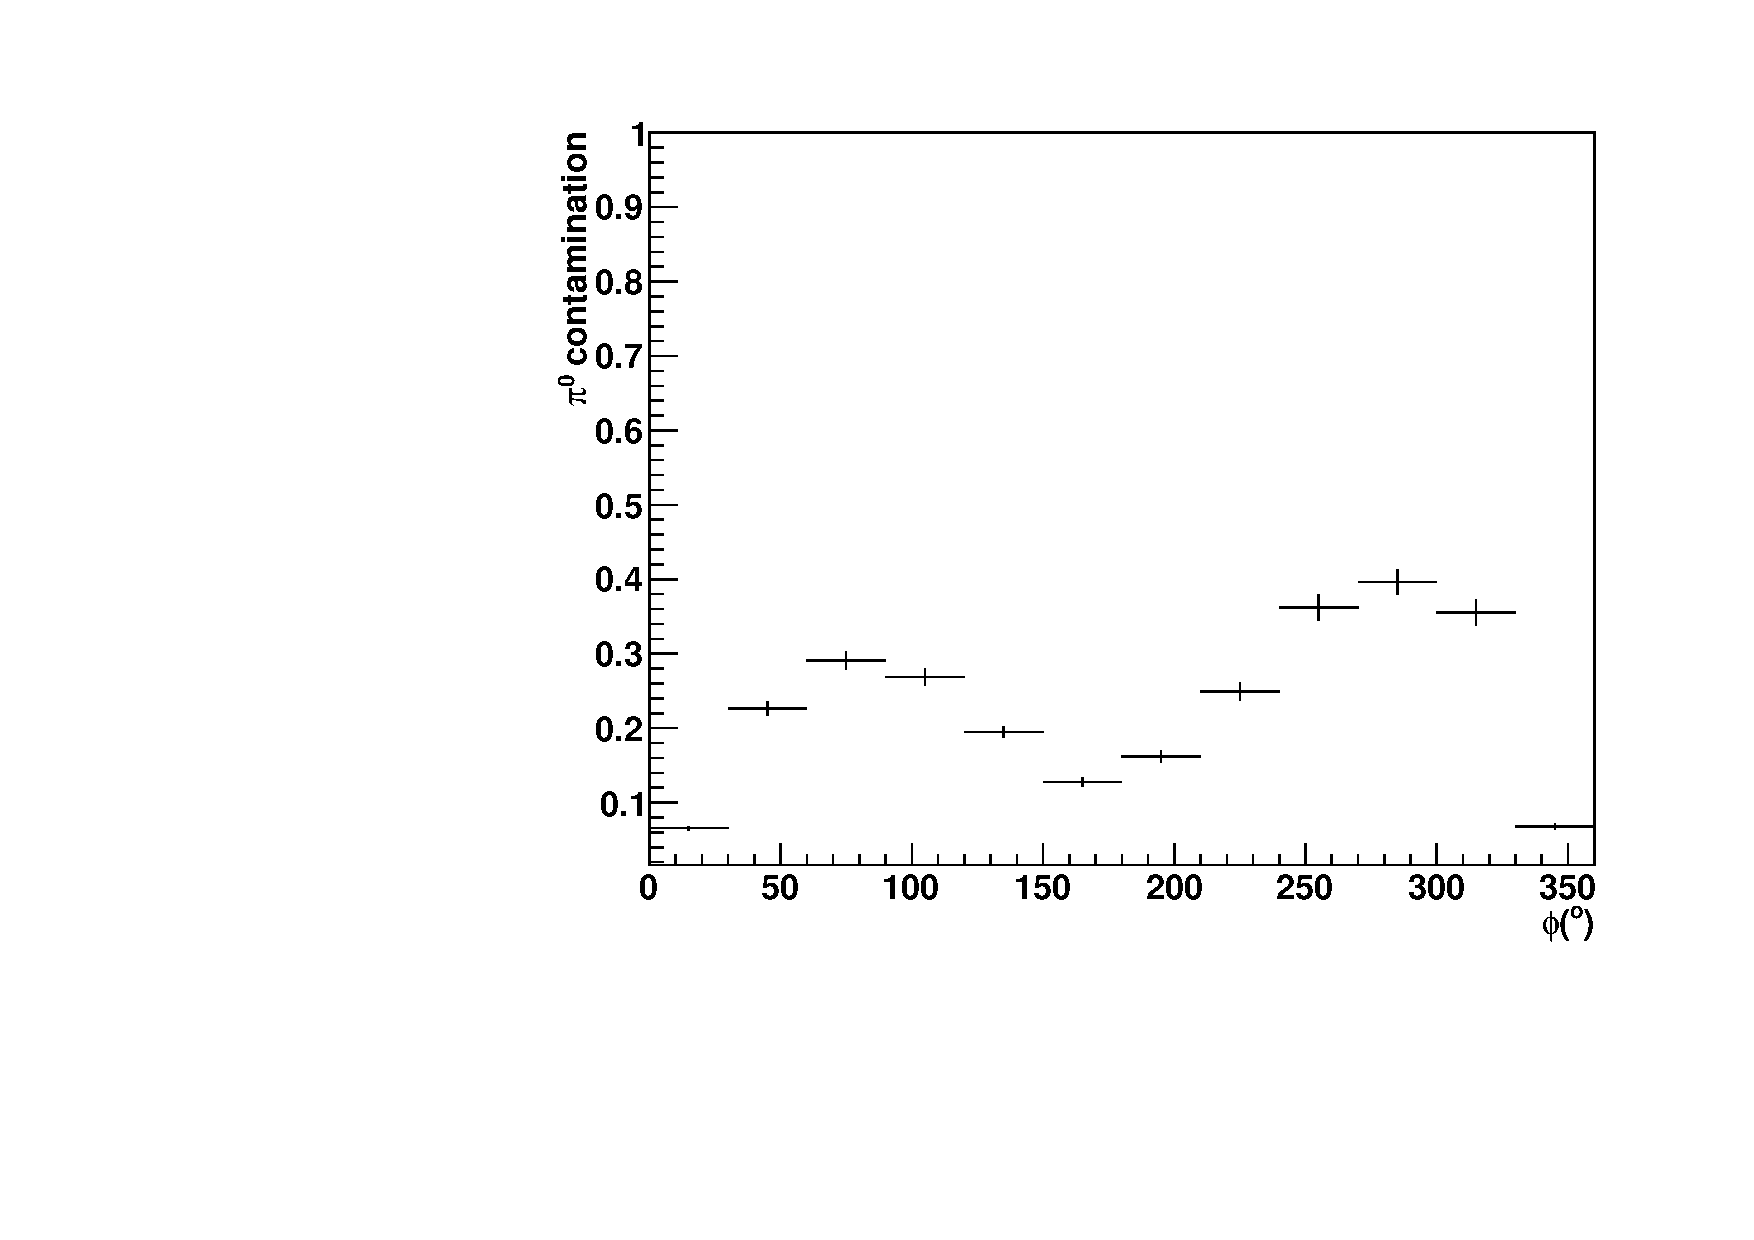
\includegraphics[width=80mm]{pi0_integrated_100days_noFT.pdf}
\caption [Expected $\pi^0$ contamination fraction as a function of $\phi$]
{Expected $\pi^0$ contamination fraction for the proposed experiment, defined as $\frac{N_{\pi^{0} 1\gamma}}{N_{en\gamma}}$, as a function of $\phi$ and integrated over the other kinematic variables. }
\label{ndvcs-pi0}
\end{center}
\end{figure}

An exploratory nDVCS analysis on the ND$_3$ subset (``part C'') of the CLAS
eg1-dvcs data-set is underway \cite{daria_eg1dvcs}. In spite of the very poor
statistics and the far from optimal neutron reconstruction in the CLAS
EC calorimeters, a selection of the nDVCS final state has been possible.
Figure~\ref{ndvcs_daria} shows the same exclusivity variables as are plotted in
Fig.~\ref{dvcs_excl}, obtained after applying nDVCS selection cuts to the $en\gamma$ event sample, which were optimised for the eg1-dvcs data. The similarities with our simulations are remarkable, especially considering that no nuclear background was subtracted from the distributions of Fig.~\ref{ndvcs_daria}, which gives confidence in this data-selection technique for the proposed experiment. Additionally, the effect of nuclear background subtraction can be seen in Fig.~\ref{daria_sub}, which shows the missing mass squared from $en\to enX$ before and after subtraction of opportunely scaled distributions obtained with carbon data,
and in Fig.~\ref{daria_sub_fit} , displaying the carbon-subtracted $m_{X}^{2}$ 
distribution from $en \to en\gamma X$. The figure indicates that a good selection of the $en\gamma$ final state has been possible even within the limitations 
of the eg1-dvcs experiment and illustrate the applicability of the 
technique to the proposed experiment.

\begin{figure}
\begin{center}
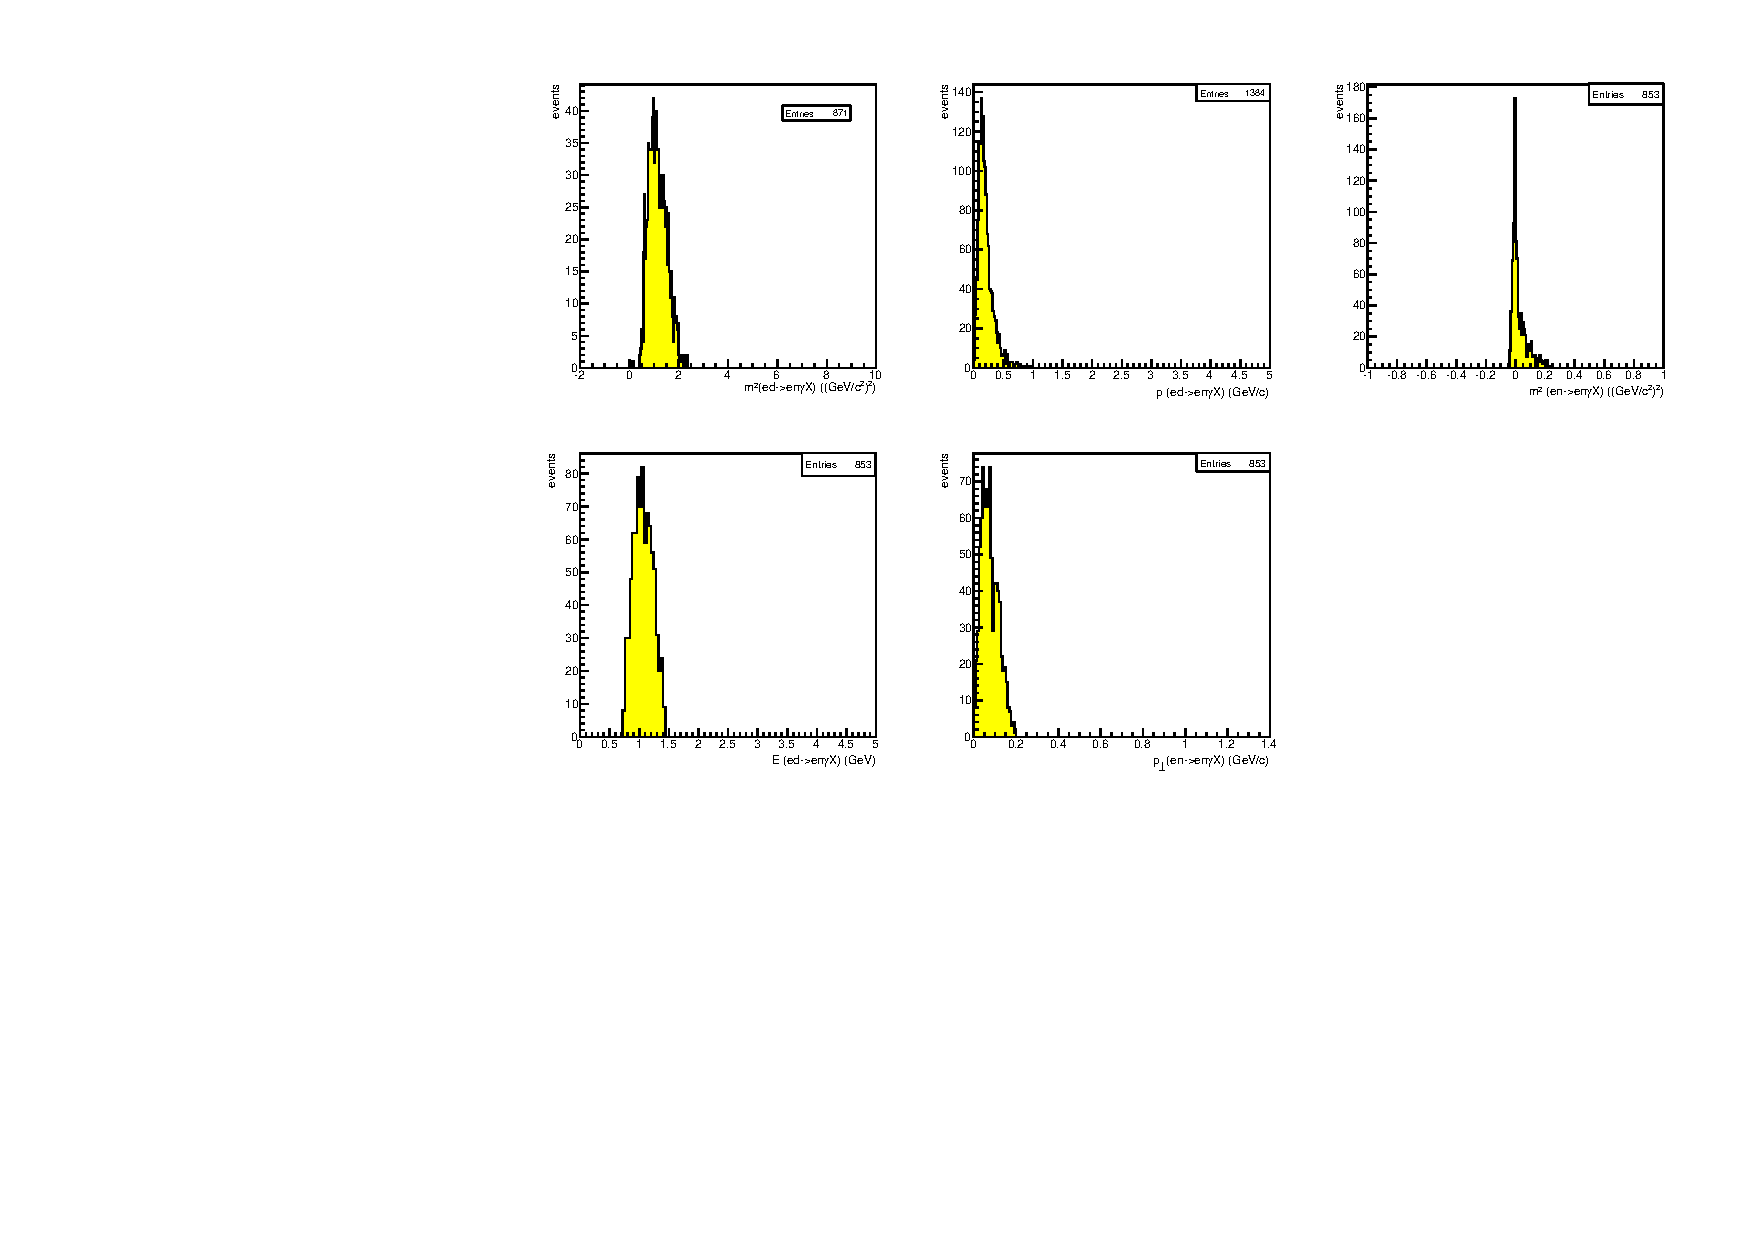
\includegraphics[width=120mm]{nDVCS_data_exclusivity.pdf}
\caption[nDVCS, CLAS eg1-dvcs analysis]
{nDVCS analysis of the CLAS eg1-dvcs data set, after exclusivity cuts: DVCS exclusivity variables, same as Fig.\ref{dvcs_excl}.}
\label{ndvcs_daria}
\end{center}
\end{figure}

\begin{figure}
\begin{center}
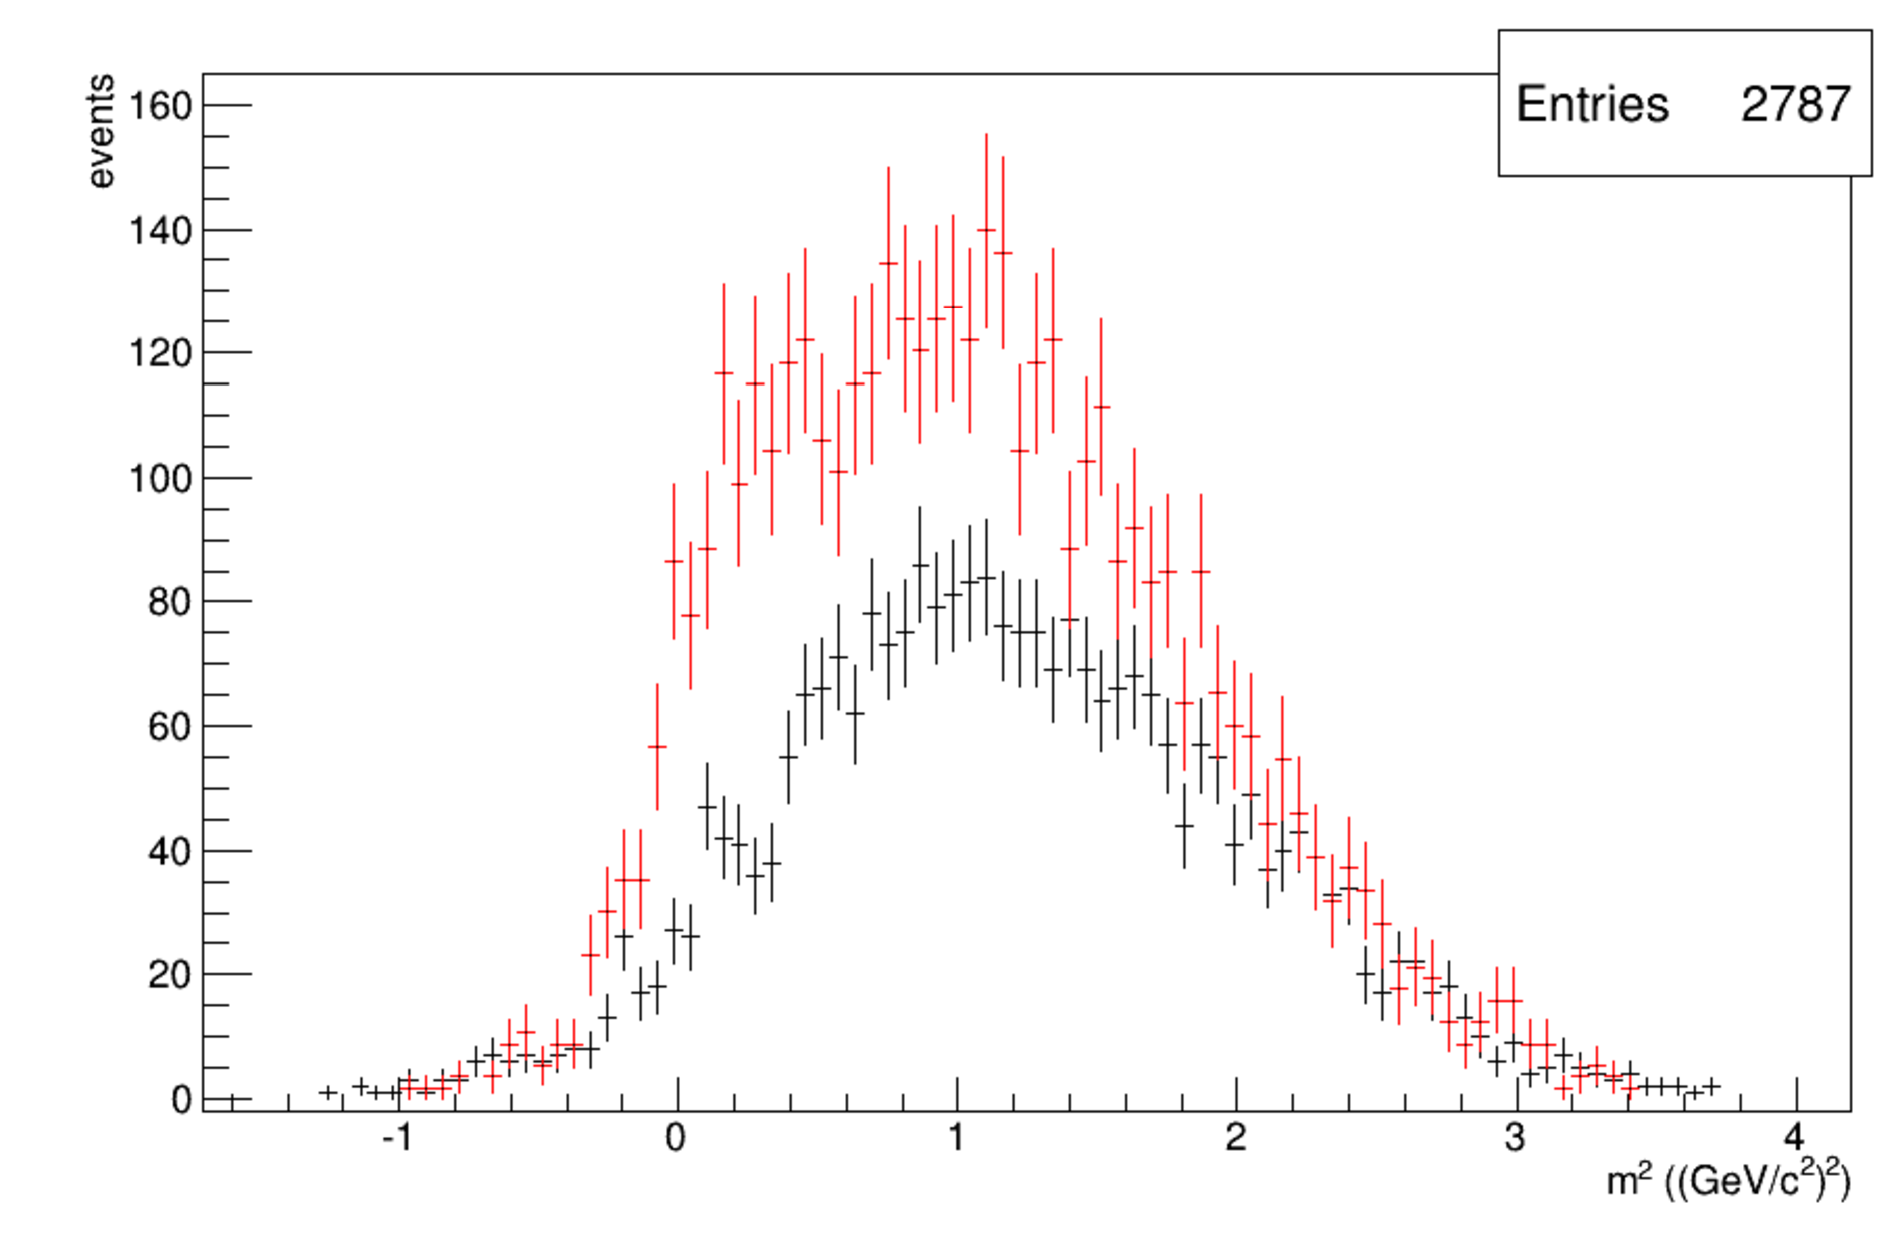
\includegraphics[width=80mm]{mm2_en.pdf}
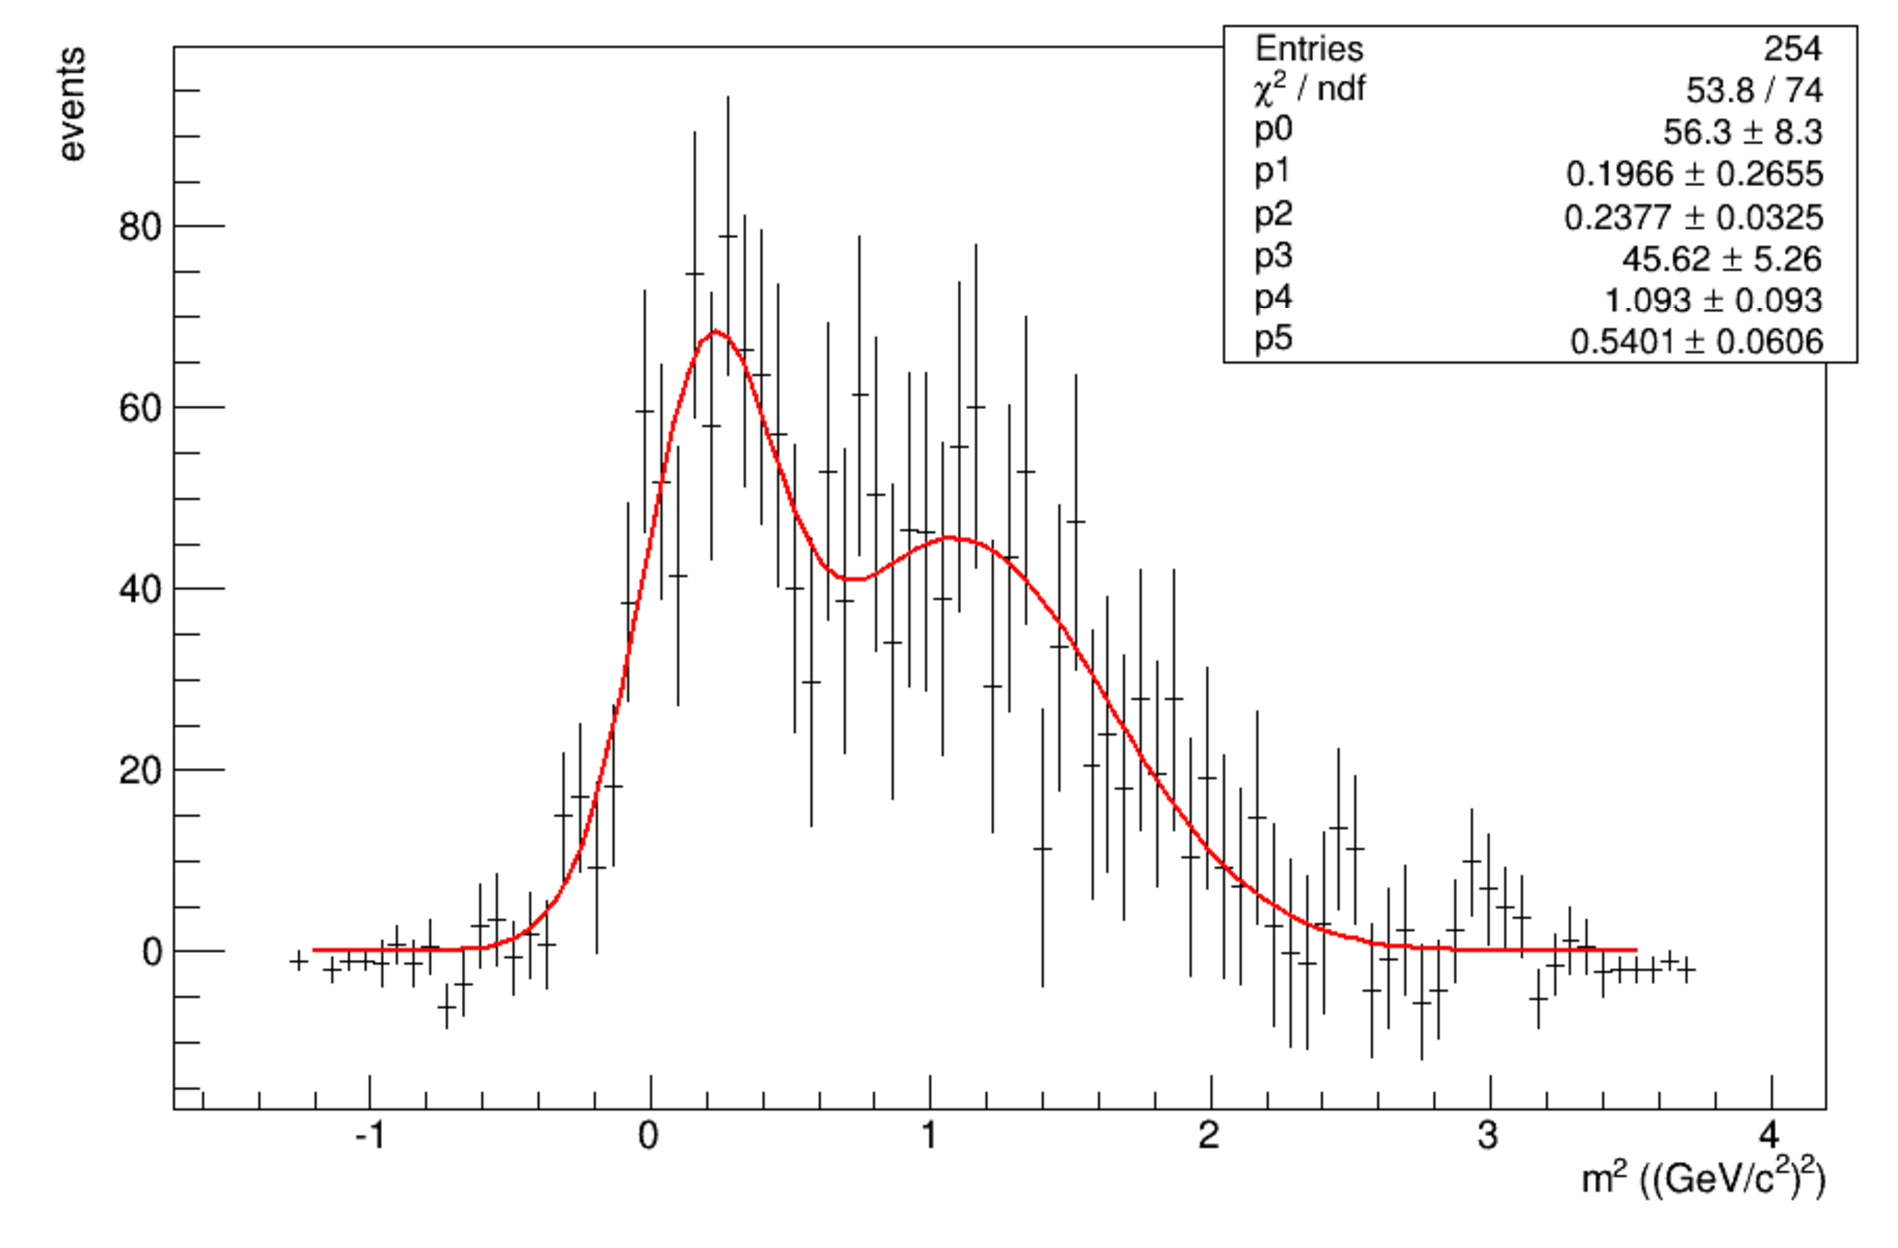
\includegraphics[width=80mm]{mm2_en_fit.pdf}
\caption 
{nDVCS analysis of the CLAS eg1-dvcs data set. Top: squared missing mass of $X$ in $en\to enX$, with ND$_{3}$ (red) and carbon (black); bottom: after carbon subtraction, a peak near 0 appears. }   
\label{daria_sub}
\end{center}
\end{figure}

\begin{figure}
\begin{center}
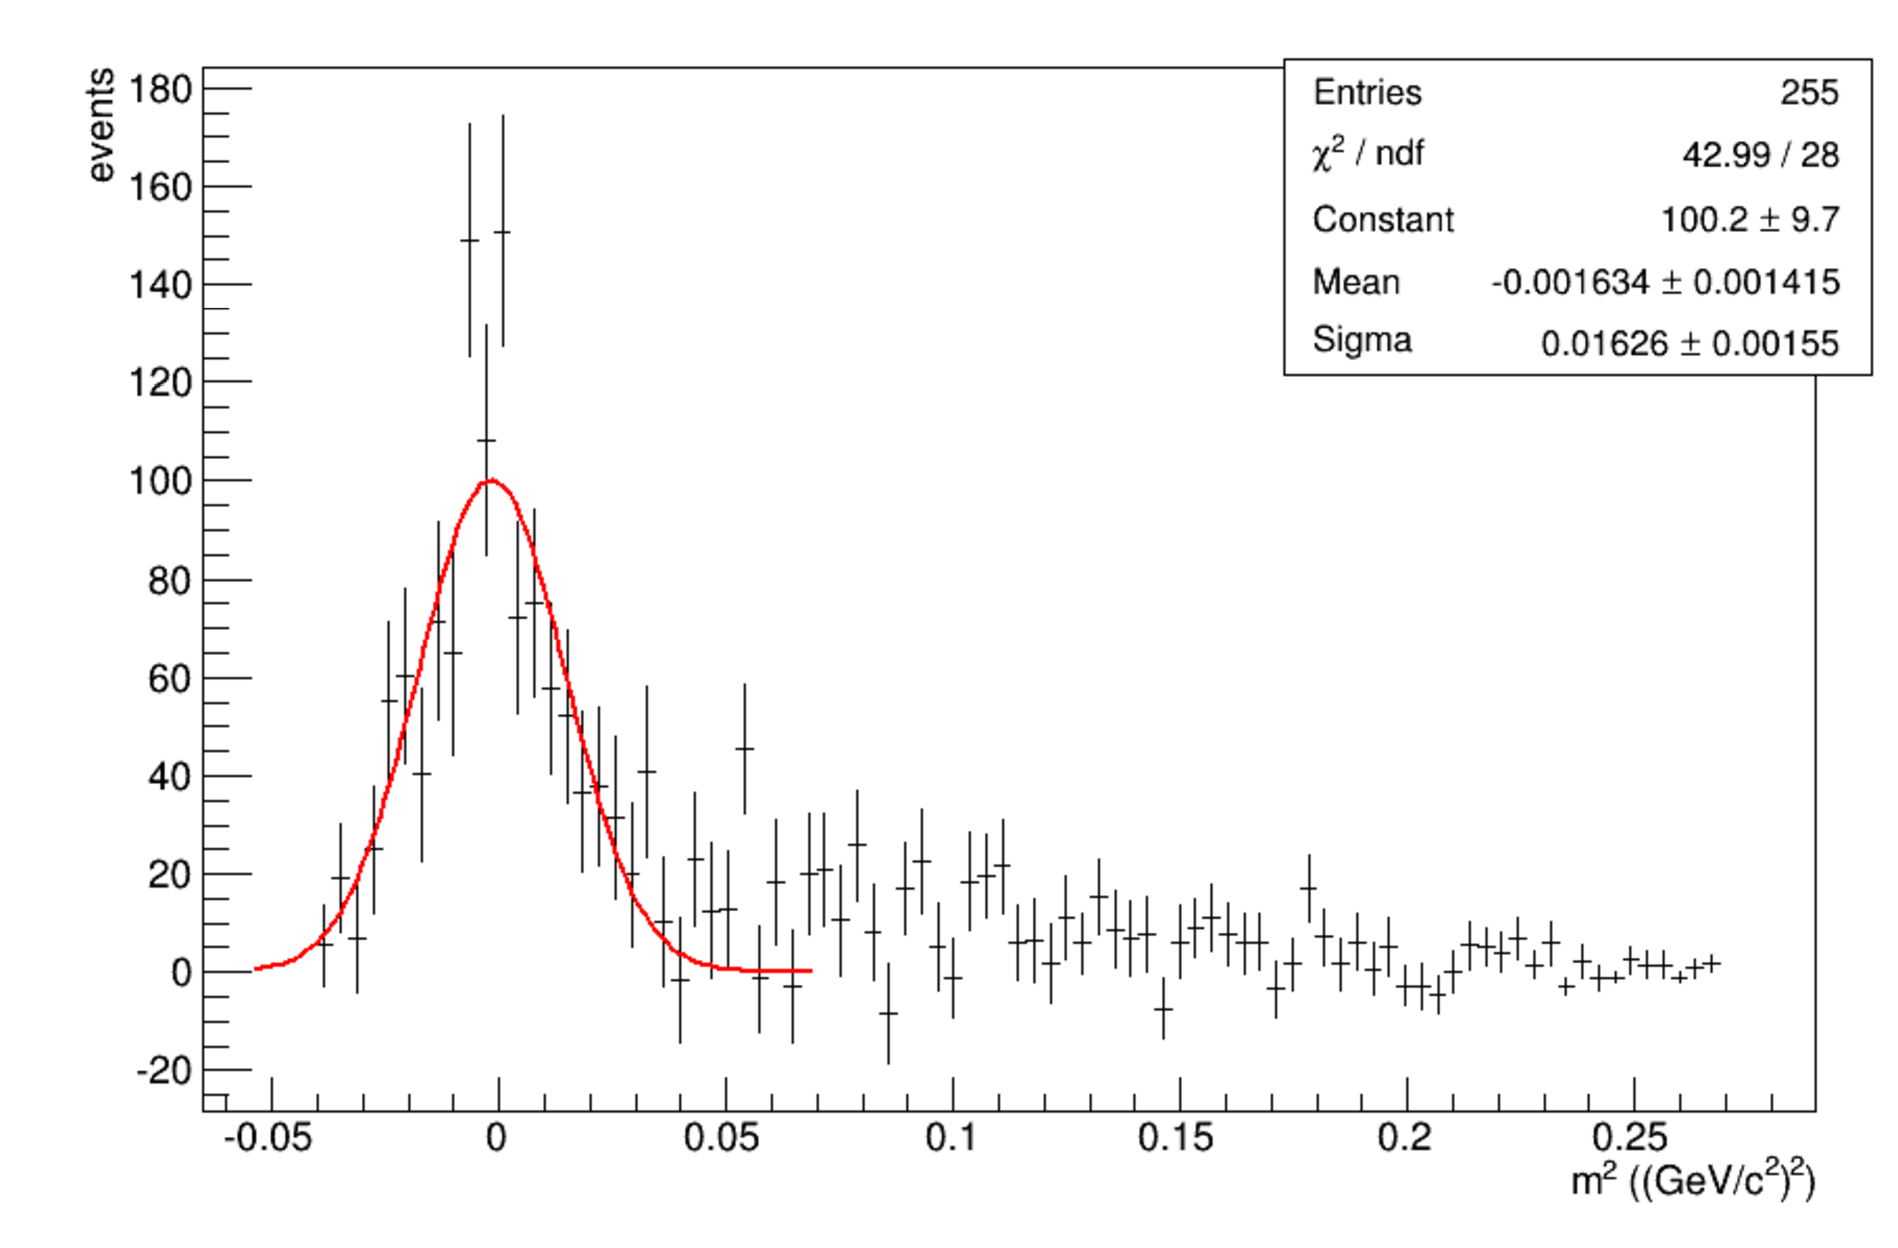
\includegraphics[width=80mm]{mm2_eng_fit.pdf}
\caption
{nDVCS analysis of the CLAS eg1-dvcs data set: squared missing mass of $X$ in $en\to en\gamma X$, after exclusivity cuts and carbon subtraction.}
\label{daria_sub_fit}
\end{center}
\end{figure}

\section{Neutral pion background }\label{sec_pi0_back}

Once the events containing one electron, one active neutron and one energetic photon are selected, and no other charged particles are detected in CLAS12, the nDVCS/BH final state can be isolated by cutting on the $en\gamma$ missing mass and the other exclusivity variables. These selection criteria will eliminate the majority of the competing channels, such as, for instance, charge-exchange reactions on the proton, where a positively charged meson (mostly a $\pi^+$) is emitted along with the neutron. 
However, due to the finite resolutions of the detectors, the final event sample will still be contaminated by $en\gamma$ events coming from the $en\pi^0(p)$ channel, where one photon from the $\pi^0$ decay is detected in the forward part of CLAS12 while the other escapes detection. This contamination will be evaluated and subtracted as was done in previous DVCS CLAS analyses \cite{fx,erin,pisano,hs}, by extracting exclusive $en\pi^0(p)$ events --- detecting both decay photons --- from the data, and using Monte Carlo simulations to evaluate the ratio of acceptances of $\pi^0$ events with 1 and 2 photons detected. The final number of nDVCS/BH events, in each 4-dimensional bin, will be obtained as:

\begin{eqnarray}
N_{DVCS}(Q^2,x_B,-t,\phi)=N_{en\gamma}(Q^2,x_B,-t,\phi)-N_{\pi^0 1\gamma}(Q^2,x_B,-t,\phi)
\end{eqnarray}
where
\begin{eqnarray}\label{pi0_formula}
N_{\pi^0 1\gamma}(Q^2,x_B,-t,\phi)=N^{data}_{\pi^0}(Q^2,x_B,-t,\phi)\cdot \frac{N^{MC}_{\pi^0 1\gamma}(Q^2,x_B,-t,\phi)}{N^{MC}_{\pi^0 2\gamma}(Q^2,x_B,-t,\phi)}
\end{eqnarray}

As an example, Fig.~\ref{pi0_eg1dvcs} shows the elements contributing to the $\pi^0$ background subtraction, as were evaluated for the extraction of the TSA in the CLAS eg1-dvcs analysis, for two particular kinematic bins in $(Q^2, x_B, -t)$. Note that the impact on the final asymmetry of the background subtraction is quite small: an average effect of roughly 10\%, relative to the value of the TSA at $90^{\circ}$, was estimated for this data set. In fact, what will impact the final asymmetries is not the size of the contamination itself, but the point-by-point difference of contamination for positive and negative target (or beam-target) polarization. 

\begin{figure}  
\begin{center}
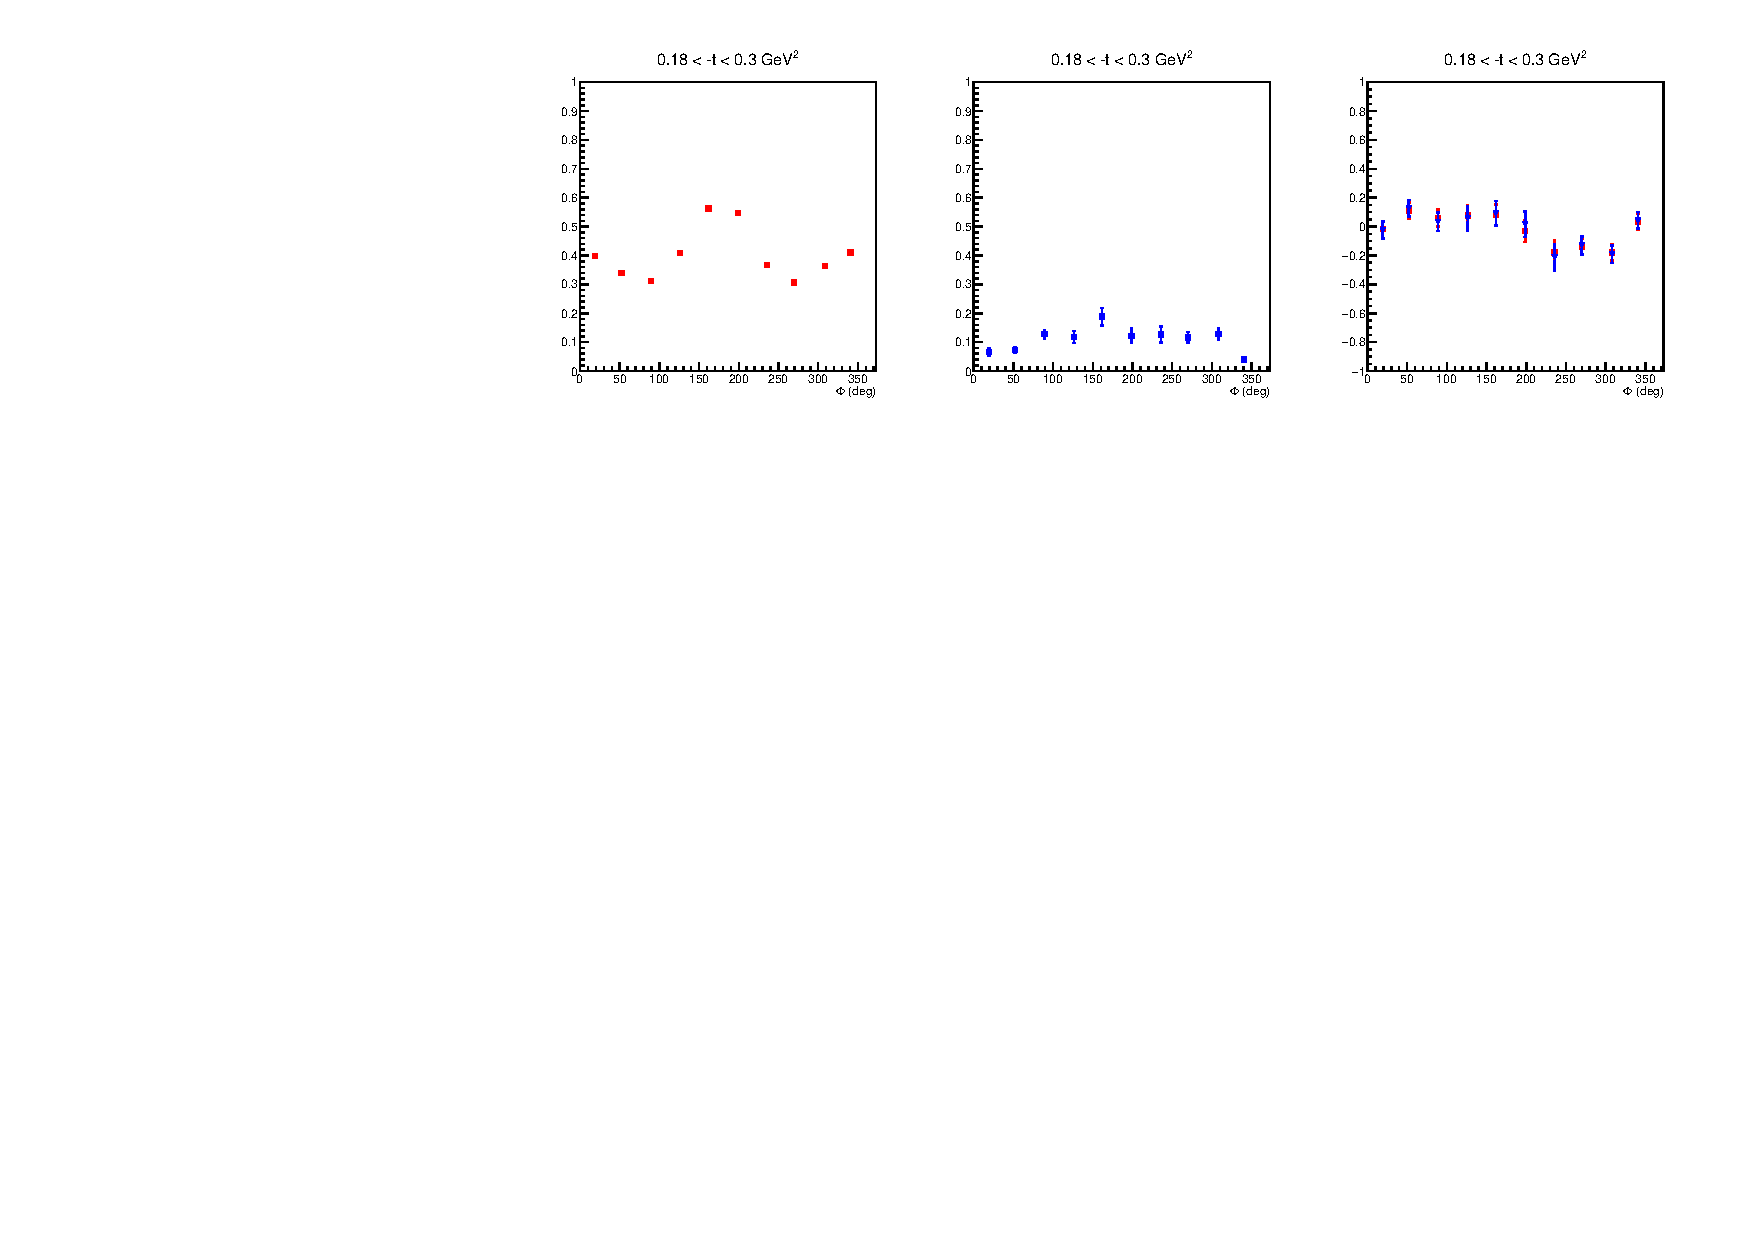
\includegraphics[width=140mm]{pi0_cont_tsa.pdf}
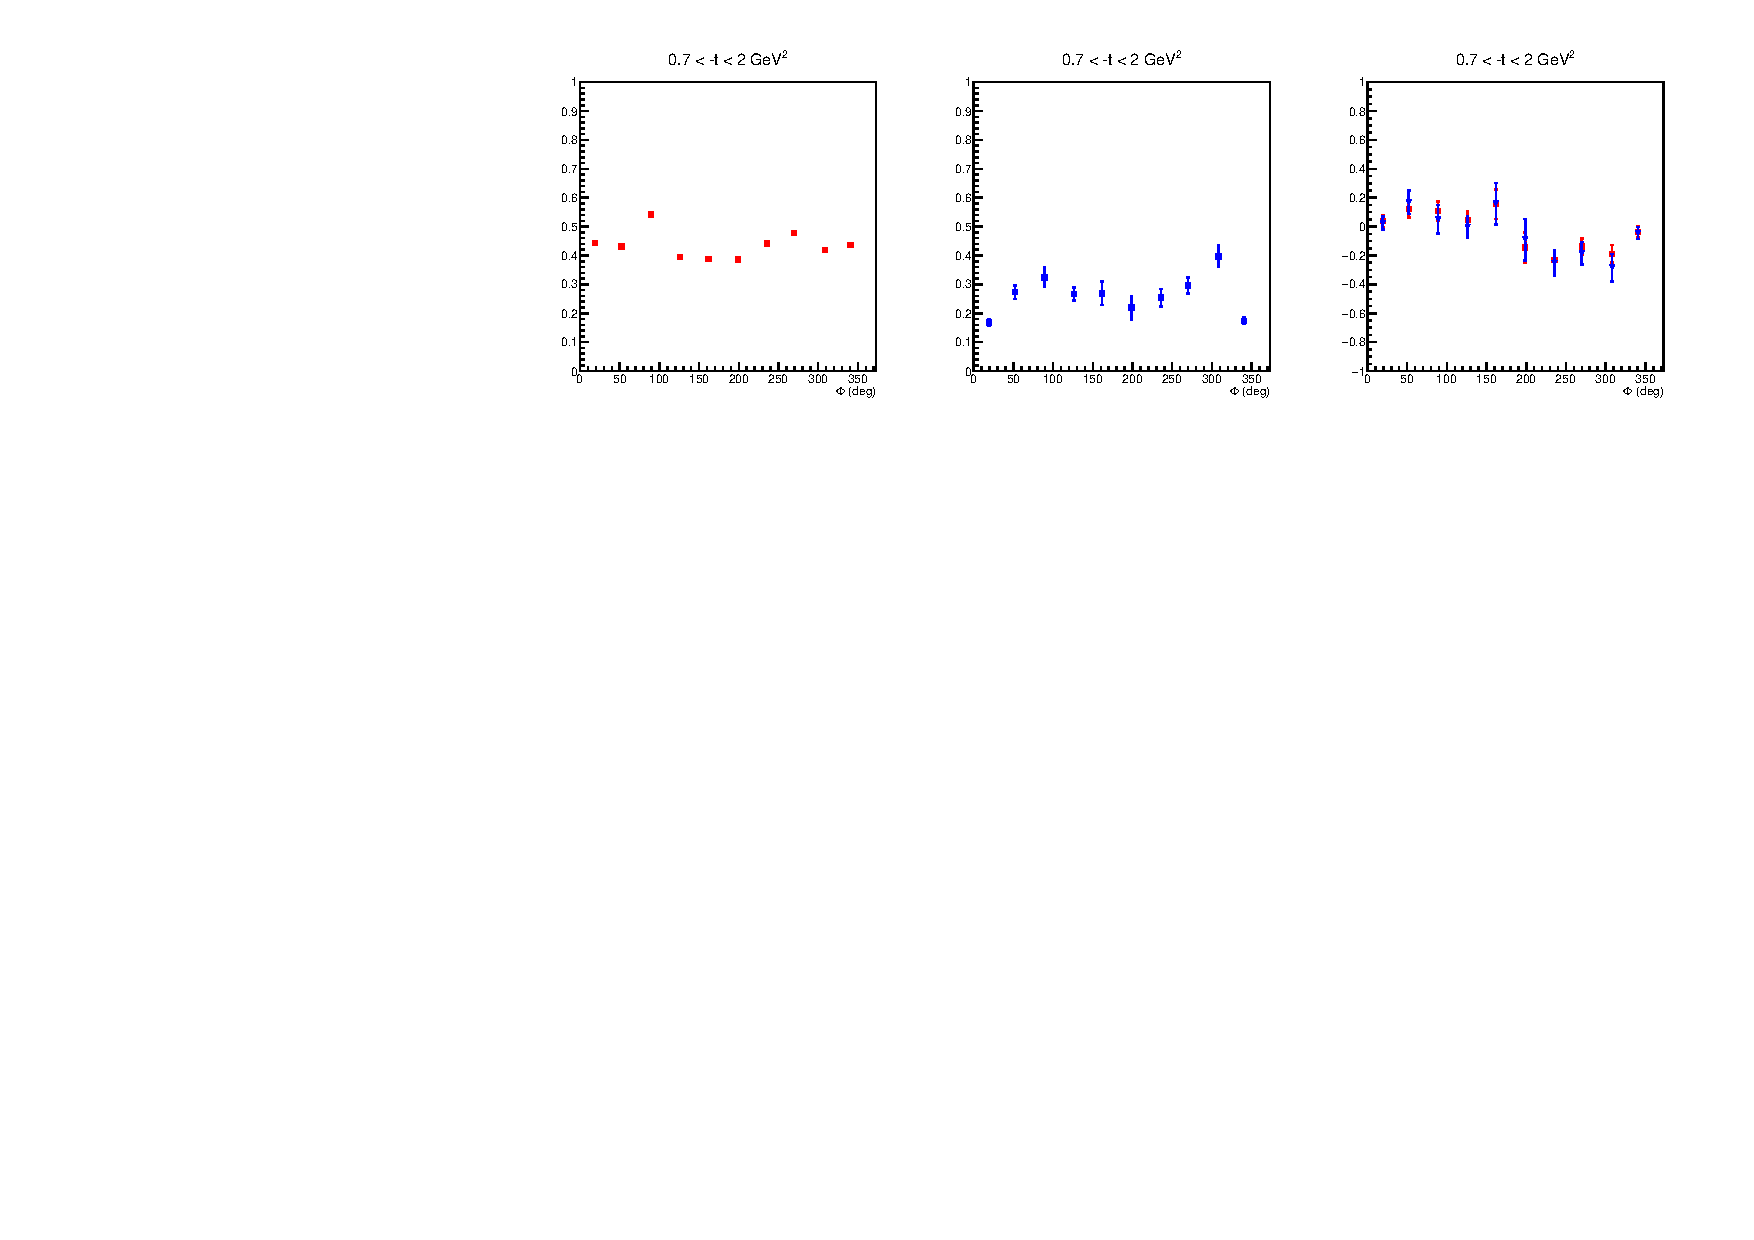
\includegraphics[width=140mm]{bin_q20_xb3_t3.pdf}
\caption [pDVCS results from the eg1-DVCS CLAS dataset]
{Plots from the proton-DVCS analysis of the eg1-DVCS CLAS dataset \cite{pisano}, for two different kinematic bins (top and bottom). Left: Acceptance ratio "$\frac{1 \gamma}{2 \gamma}$"; middle: $\pi^0$ contamination fraction; right: target-spin asymmetry before (red) and after (blue) $\pi^0$ background subtraction.}
\label{pi0_eg1dvcs}
\end{center}
\end{figure}
%
The proton-DVCS analysis of the eg1-dvcs NH$_{3}$ dataset showed that a combination of optimized cuts on the exclusivity variables, designed to minimise the background, and the simulation- and data- based subtraction of Eq.~\ref{pi0_formula} to remove the remaining contamination was a sound technique. In terms of systematics, the asymmetries were minimally affected even when the background estimation was artificially varied by 30\%. This is important also because it shows how little this procedure depends on the Monte-Carlo model adopted. 

\section{Dilution factor}\label{sec_dilution}
For both the nDVCS and $en\pi^0$ final states, dilution factors are necessary to correct the experimental yields for the contribution from the scattering on the unpolarized nitrogen of ND$_3$. The dilution factor, that will be determined using data taken on ND$_3$ and on ${}^{12}$C targets, is defined as
\begin{equation}
D_f = 1-c\cdot\frac{N_{{}^{12}{\rm C}}}{N_{{}^{14}{\rm ND}_3}} \label{eq_dilution}.
\end{equation}
Here, $N_{{}^{12}{\rm C}}$ is the number of events, normalized by the corresponding Faraday-cup counts, obtained from a carbon target and surviving all of the nDVCS (or $en\pi^0$) selection cuts, while $N_{{}^{14}{\rm ND}_3}$ is the number of events, likewise normalized and passing the same series of cuts, originating from ND$_3$. The factor $c$ accounts for the different luminosities of the two sets of data, which also take into account the different areal densities of the materials 
present at the target level for the two kinds of runs (ND$_3$ in the numerator, ${}^{12}$C in the denominator). 
For the eg1-dvcs experiment, it was found that the dilution factor, which, for pDVCS was determined to be around 0.9, does not display any sizeable dependence on any of the four kinematic variables describing the DVCS process. 
Adopting the same ratio as in eg1-dvcs, we estimate that acquiring ten times less events on ${}^{12}$C than on ND$_3$ should provide a sufficient count rate of carbon events to estimate the dilution factor at a satisfactory level of precision. A value of about 0.8 was obtained in recent studies of exclusive channels on ND$_3$, still using the eg1-dvcs dataset \cite{peter_exclusive}.
%As the dilution factor depends strongly on the exclusivity cuts, a conservative estimate of 0.7 is adopted for $D_f$ to produce the projected asymmetries of this proposal (Section~\ref{sec_countrate}). 

\section{Accidentals in the CND}\label{sec_accidentals}

In order to evaluate the rate of accidentals being reconstructed as a false neutron in the CND in coincidence with an $e\gamma$ event detected in CLAS12, GEMC simulations have been run in the following conditions \cite{raffa,proposal}: the primary electron has been generated going forward (to simulate the real hadronic event), plus 7500 other electrons have been thrown, distributed in a 124 ns window in bunches 4 ns apart, originating 10 cm upstream of the target. 7500 is approximately the number of beam electrons that would pass through our target in a 124 ns time window at the nominal CLAS12 luminosity. 124 ns is the typical time window of the DAQ expected for CLAS12, which corresponds to one event in CLAS12. These electrons then interact with the target itself, producing an electromagnetic and hadronic background hitting the neutron detector. The simulations were produced twice, using two different "physics lists" from GEANT4: electromagnetic plus hadronic processes ("EM-HAD"), and electromagnetic only (EM). The output of the simulations has been analyzed using the CND neutron-reconstruction algorithm. For each event, we selected the hit with the shortest time of flight which had a deposited energy above our chosen threshold (2~MeV) and below the maximum allowed time (9~ns). The reference time was chosen as that corresponding to the central beam bunch. Given the tight timing cuts that are imposed when reconstructing neutrons in the CND, we estimate that only slow neutrons ($p\sim 0.2$ GeV) from the previous bunch or photons from the following bunch could be accidentally registered as originating from the bunch in question. The momentum of the chosen particle is reconstructed assuming that it is a neutron, and cuts are applied on its momentum ($p_{min}= 0.2$ GeV/c) and on $\beta$ ($\beta<0.95$). Since previous simulations showed us that real neutrons should only produce at most one hit in one of the three layers of the CND, particles which had a second hit in another layer along the same trajectory were also removed. 
Figure~\ref{edep_background} shows the energy distribution of the background hits in the CND before any cuts are applied for the EM (top) and EM-HAD (bottom) cases. The latter has a more important tail at higher energies. 

\begin{figure}  
\begin{center}
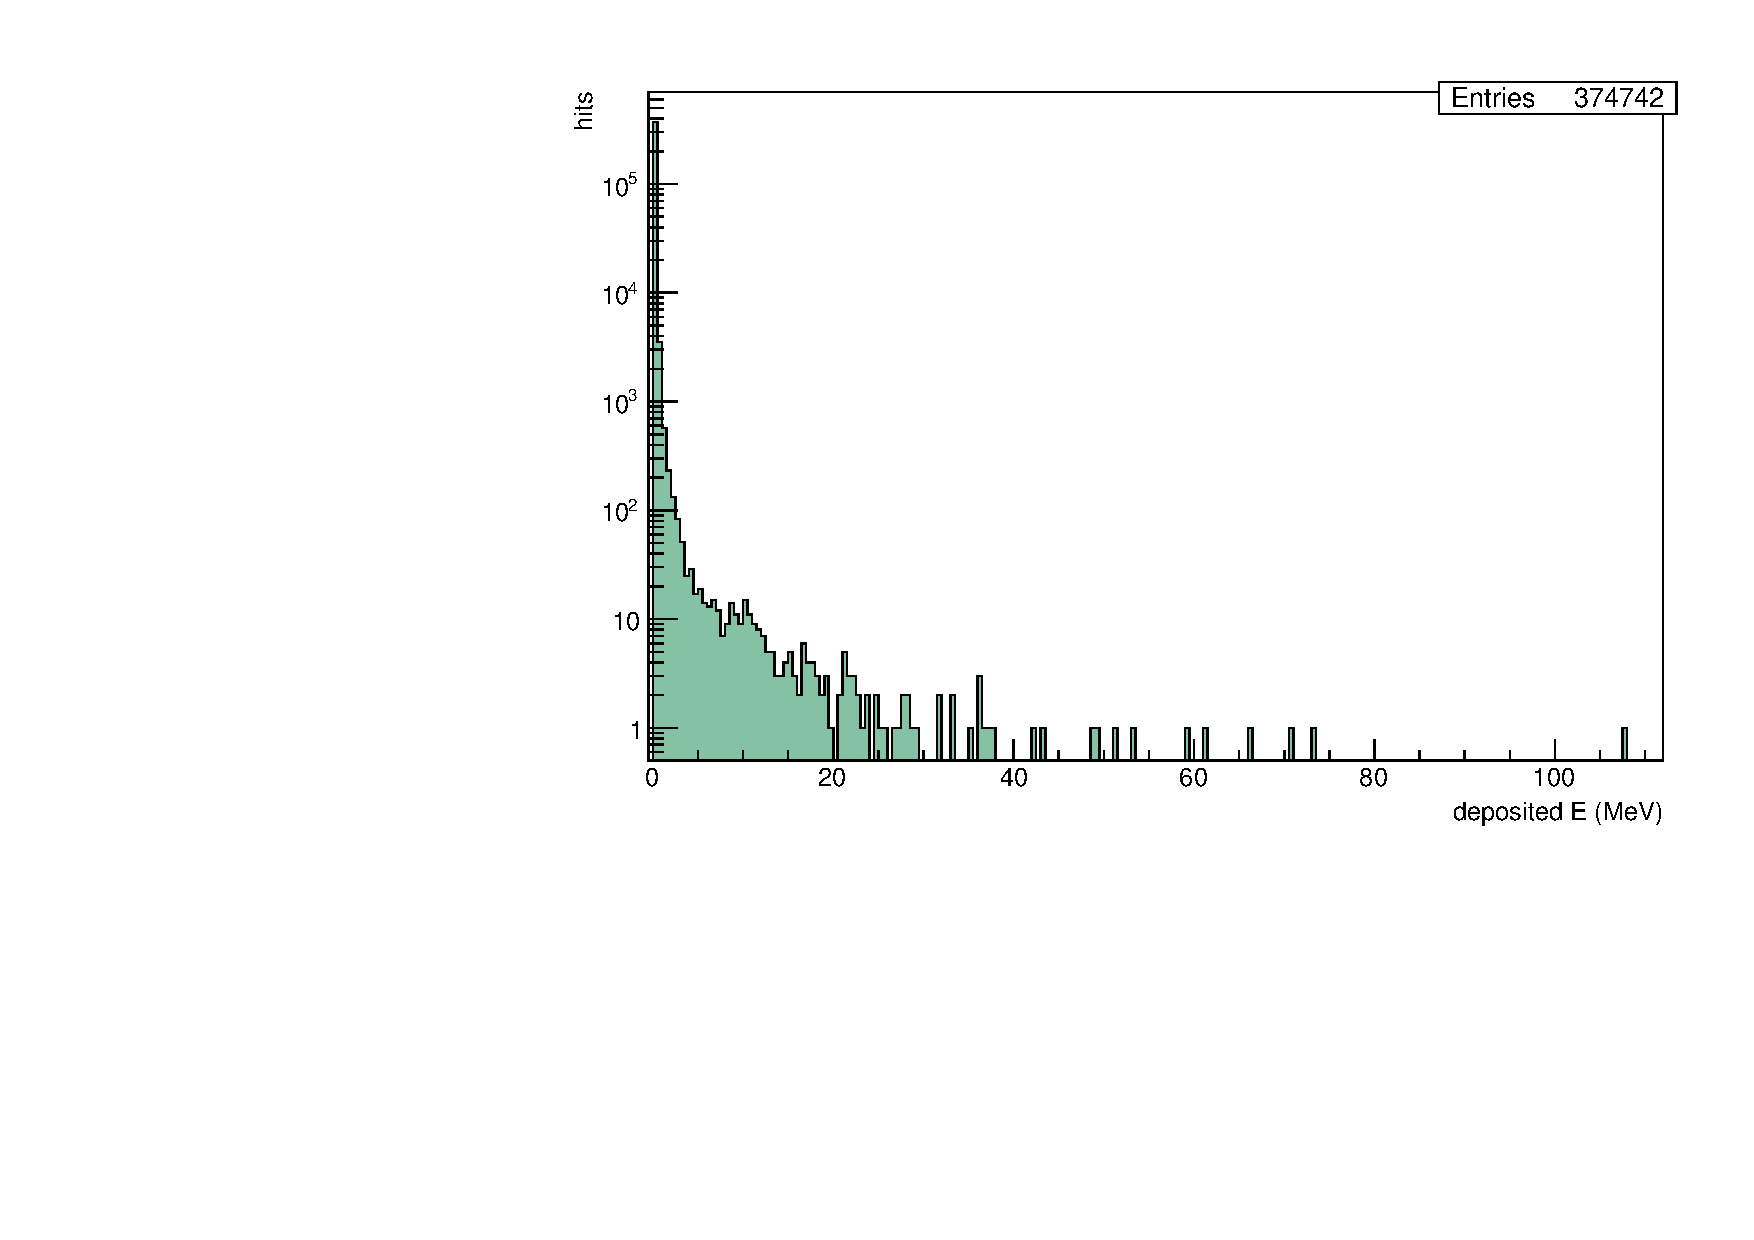
\includegraphics[width=100mm]{Egen_beforecuts_EMonly.pdf}
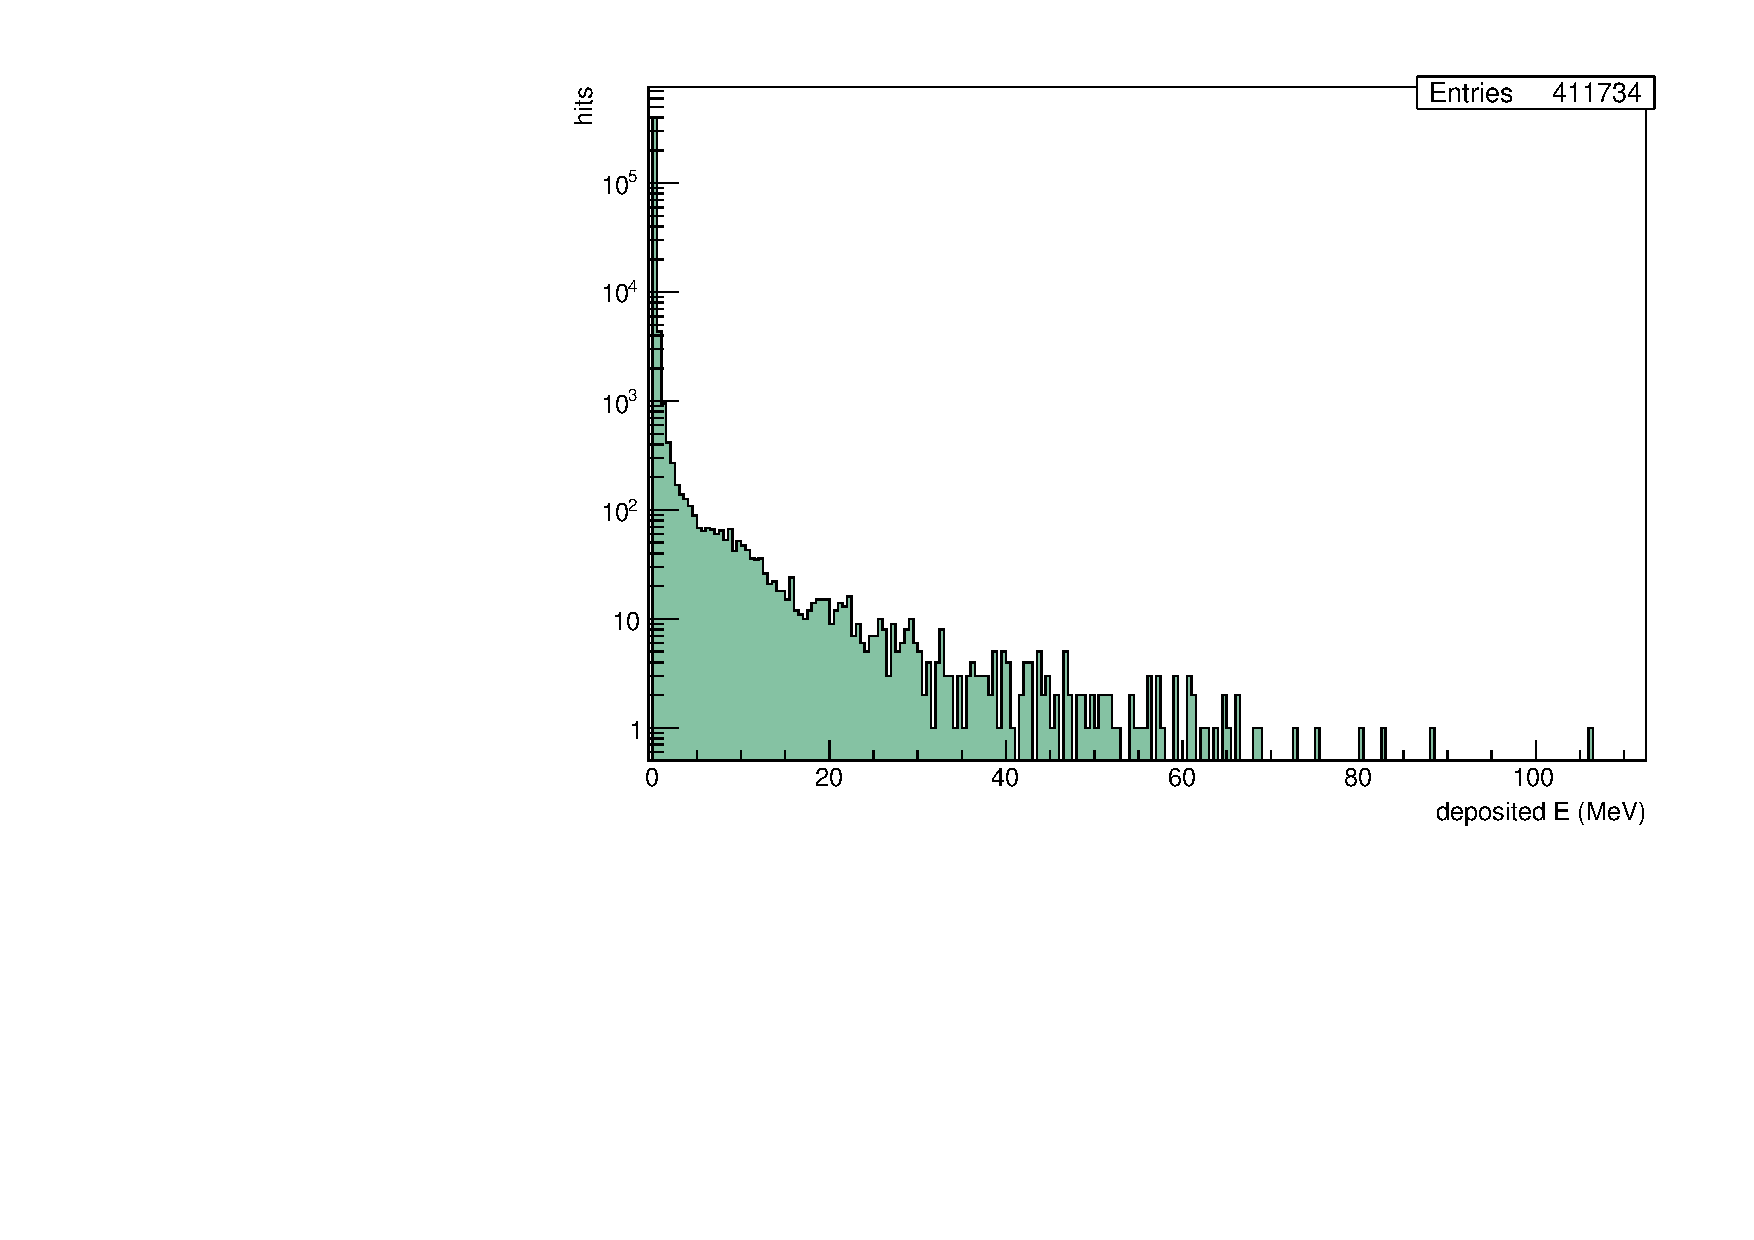
\includegraphics[width=100mm]{Egen_beforecuts_EMhad.pdf}
\caption []
{Energy deposited by the background hits in the CND, before cuts, as obtained with GEMC plus the EM physics list (top) and the EM-HAD one (bottom).}
\label{edep_background}
\end{center}
\end{figure}

The resulting probabilities that an event has a hit which passes the CND cuts are 0.0012 for the EM case and 0.01 for the EM-HAD case. Care must be taken in considering the EM-HAD probability, as there can be, on the one hand, double counting due to some of the simulated hadronic events producing actual triggers in CLAS12, and, on the other hand, uncertainties due to the GEANT4 parametrization of the physics list. The GEMC simulation of the whole CLAS12 and the full reconstruction software would be necessary to provide a more accurate estimate, but neither are available yet. The 0.01 of the EM-HAD case must therefore be regarded as a conservative upper limit. 
These hits can mimic a fake n-DVCS event by accidental coincidence with hadronic events where an electron and an energetic photon ($E_{\gamma}>2$ GeV) are detected in the forward part of CLAS12. The $e\gamma$ rate was estimated to be at most 50 Hz: the dominant process at play here is SIDIS with production of a $\pi^0$; the rate for such a process was estimated in \cite{sidis_prop} to be of 9 Hz (obtained by taking into account the factor of ~20 greater luminosity in the present experiment). Given that various kinematic cuts and the detection of both photons were required to produce that figure, we take a very conservative approach, assuming a rate for such events of the order of 50 Hz. This yields an accidental coincidence rate of the order of 0.06 Hz for the EM physics list, and 0.5 Hz for the EM+HAD physics list. These figures will be further reduced once the exclusivity cuts (Section~\ref{sec_excl_cuts}) will be applied, and will be therefore safely smaller than the expected rate for real $en\gamma$ events, which was estimated, with our event generators and FastMC, to be of 1 Hz for the present experiment. 

\section{Inclusion of the Forward Tagger}\label{ft_section}
In order to maximize the acceptance for forward-emitted photons, the compatibility of this experiment with the inclusion of the Forward Tagger has been studied. It must be noted that this detector is already part of the setup for the approved longitudinally polarized proton-DVCS experiment for CLAS12 \cite{E1206119}. 
The design of the beamline and of the shieldings, which protect the Drift Chambers of CLAS12 from the M\o ller background produced by the beam in the target, are currently undergoing modifications and studies. The goal of these studies is to optimize the shielding performances for the various experimental configurations that will be adopted with CLAS12. The current plan within the collaboration is to leave the Forward Tagger always installed in CLAS12, and to change the type of shielding between the target and the FT depending on whether or not the FT is used in the experiment. Figure~\ref{ft_shieldings}, produced with the interactive version of GEMC, shows the two designs of the M\o ller shielding in the ``FT on'' (top) and ``FT off'' cases. 
\begin{figure}[htbp] 
   \centering
   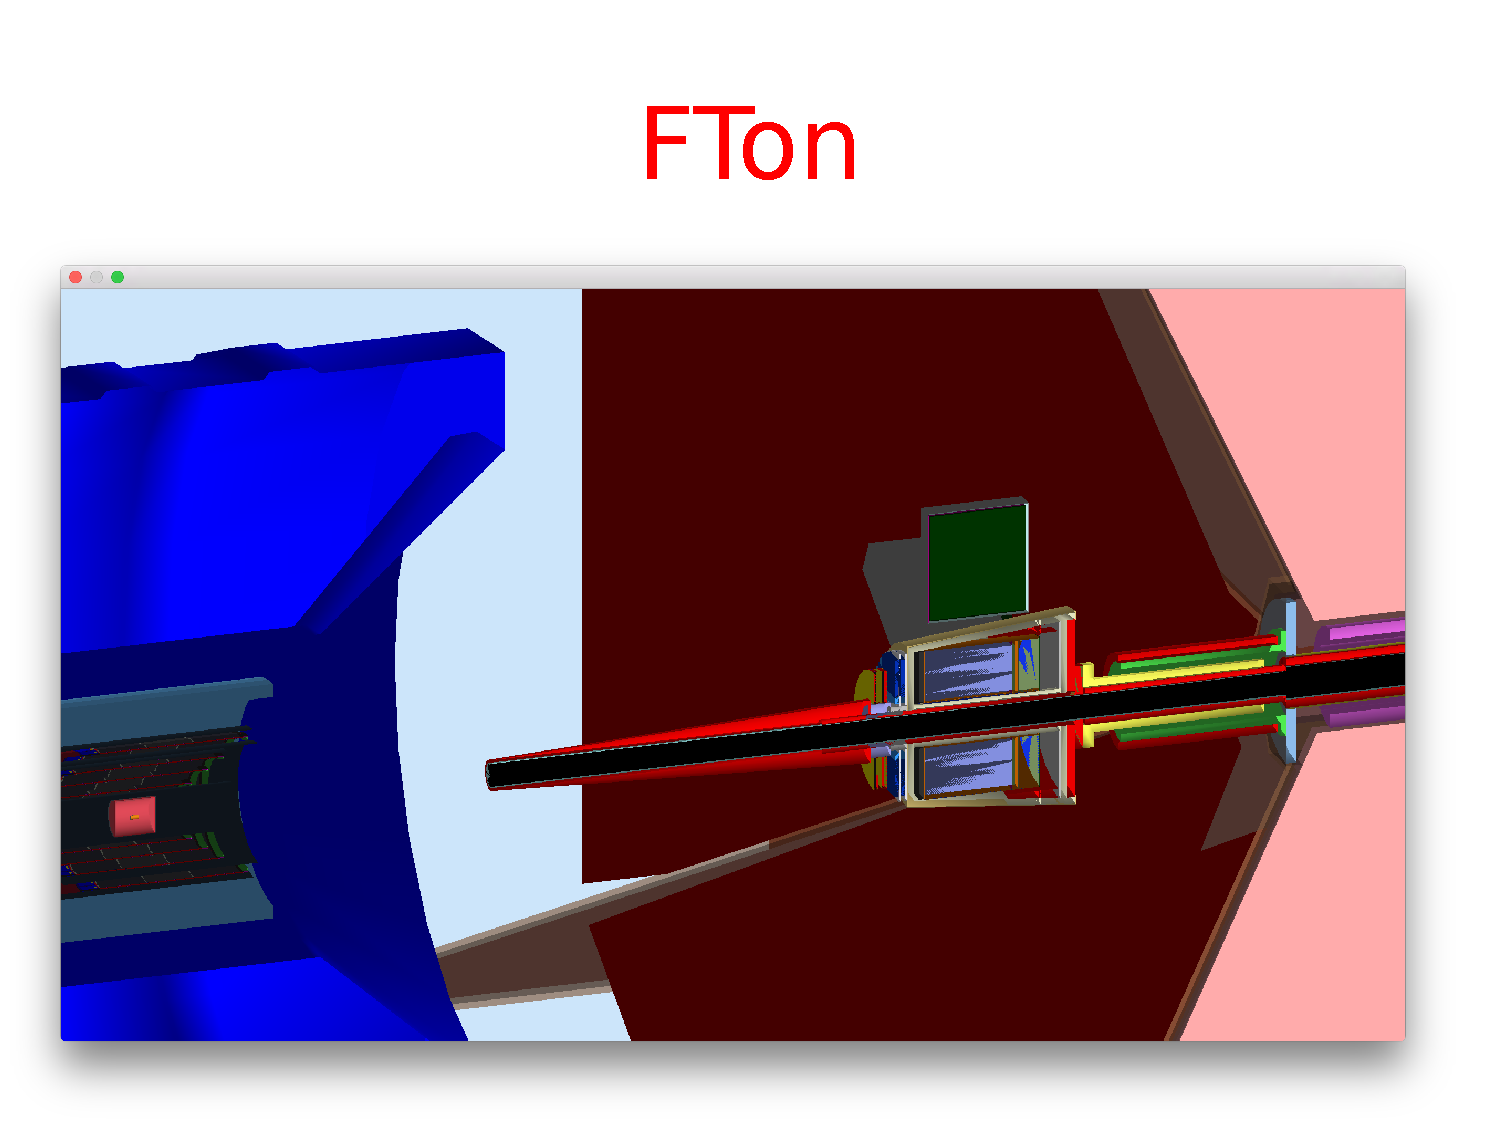
\includegraphics[width=4in]{FTon.pdf} 
   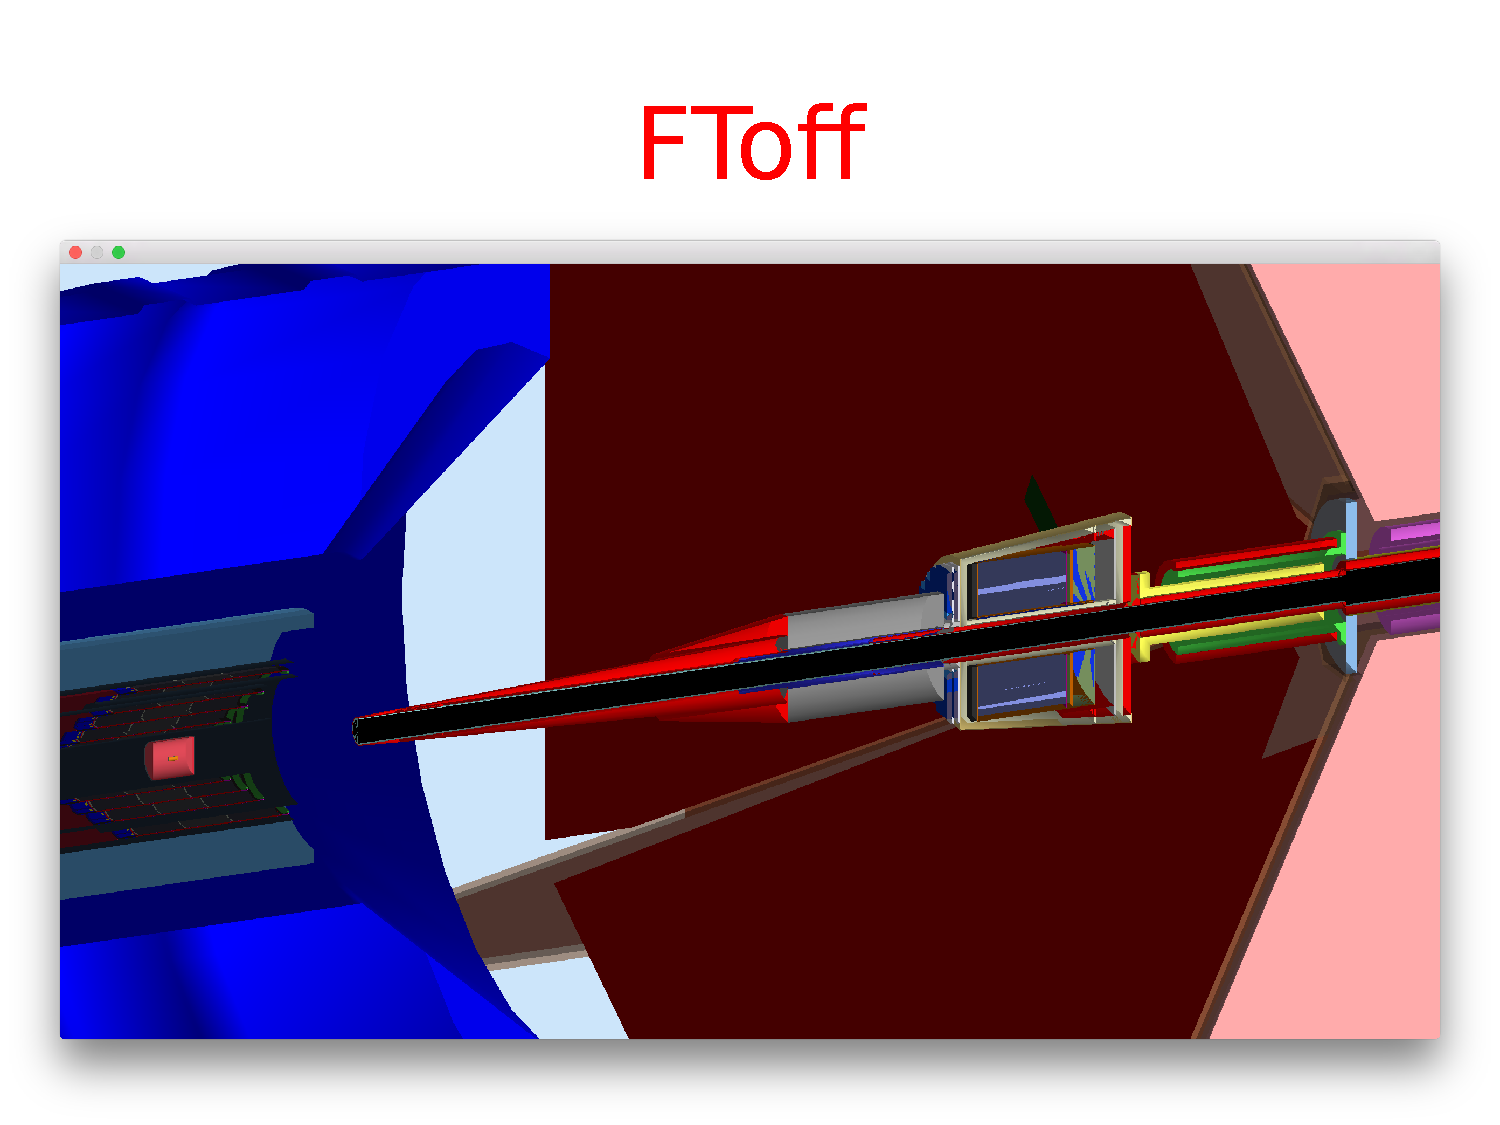
\includegraphics[width=4in]{FToff.pdf} 
   \caption{The CLAS12 M\o ller shieldings, for the ``FT on'' (top) and ``FT off'' (bottom) cases. When the FT is not used, a thicker shielding is adopted to minimize the radiation damage on the crystals.}
   \label{ft_shieldings}
\end{figure}
\subsection{DC occupancy and tracking performances at 10 nA}
Simulations were ran to test these designs, which have proven to be effective in keeping the M\o ller backgrounds low. Low background rates are necessary to ensure a high tracking efficiency. All the simulations tests performed until now were done for unpolarized targets, and thus the shieldings of Fig.~\ref{ft_shieldings} are optimized for such configuration. 
However, in the case of NH$_3$ or ND$_3$ polarized targets in order to minimize the radiation damage on the target the beam must be rastered over its surface, and this may induce higher background rates in the first region of the Drift Chambers, with respect to the unpolarized-target case. 
For the present proposal the GEMC simulation program was used to test the shieldings when the target is polarized and the beam is rastered. The polarized ND$_3$ target was implemented in GEMC as a cylindrical cell of teflon with diameter of 2.5 cm and length of 4 cm, filled with a mixture of 60\% ND$_3$ and 40\% liquid helium. The simulation was run with background events produced in a time window of 250 ns with a beam current of 10 nA, corresponding to 15625 electrons, rastered over a circular surface of 1.2 cm of radius. The four possible combinations of configurations (``with FT'', ``without FT'', ``with raster'', ``without raster'') were studied, for comparison purposes. Table ~\ref{tab:occupancy} shows the results for the occupancy in Region 1 (R1) for the four configurations, and Fig.~\ref{dc_occ} shows the occupancy for all regions of the DC for the ``with raster - with FT'' configuration, corresponding to the proposed experiment. 

\begin{table}[htbp]
   \centering
   \begin{tabular}{|c||c|} 
	\hline
      Configuration    & R1 Occupancy \\
	\hline
      FT + raster & 5.1\%\\
      FT + no raster & 2.3\%\\
      no FT + raster & 2.\%\\
      no FT + no raster & 1.8\%\\
	\hline
   \end{tabular}
   \caption{Occupancy for the first region of the CLAS12 drift chambers, obtained from GEMC simulations, for different configurations of the rastered beam and the Forward Tagger, for 10 nA of beam current.}
   \label{tab:occupancy}
\end{table}
\begin{figure}[htbp] 
   \centering
   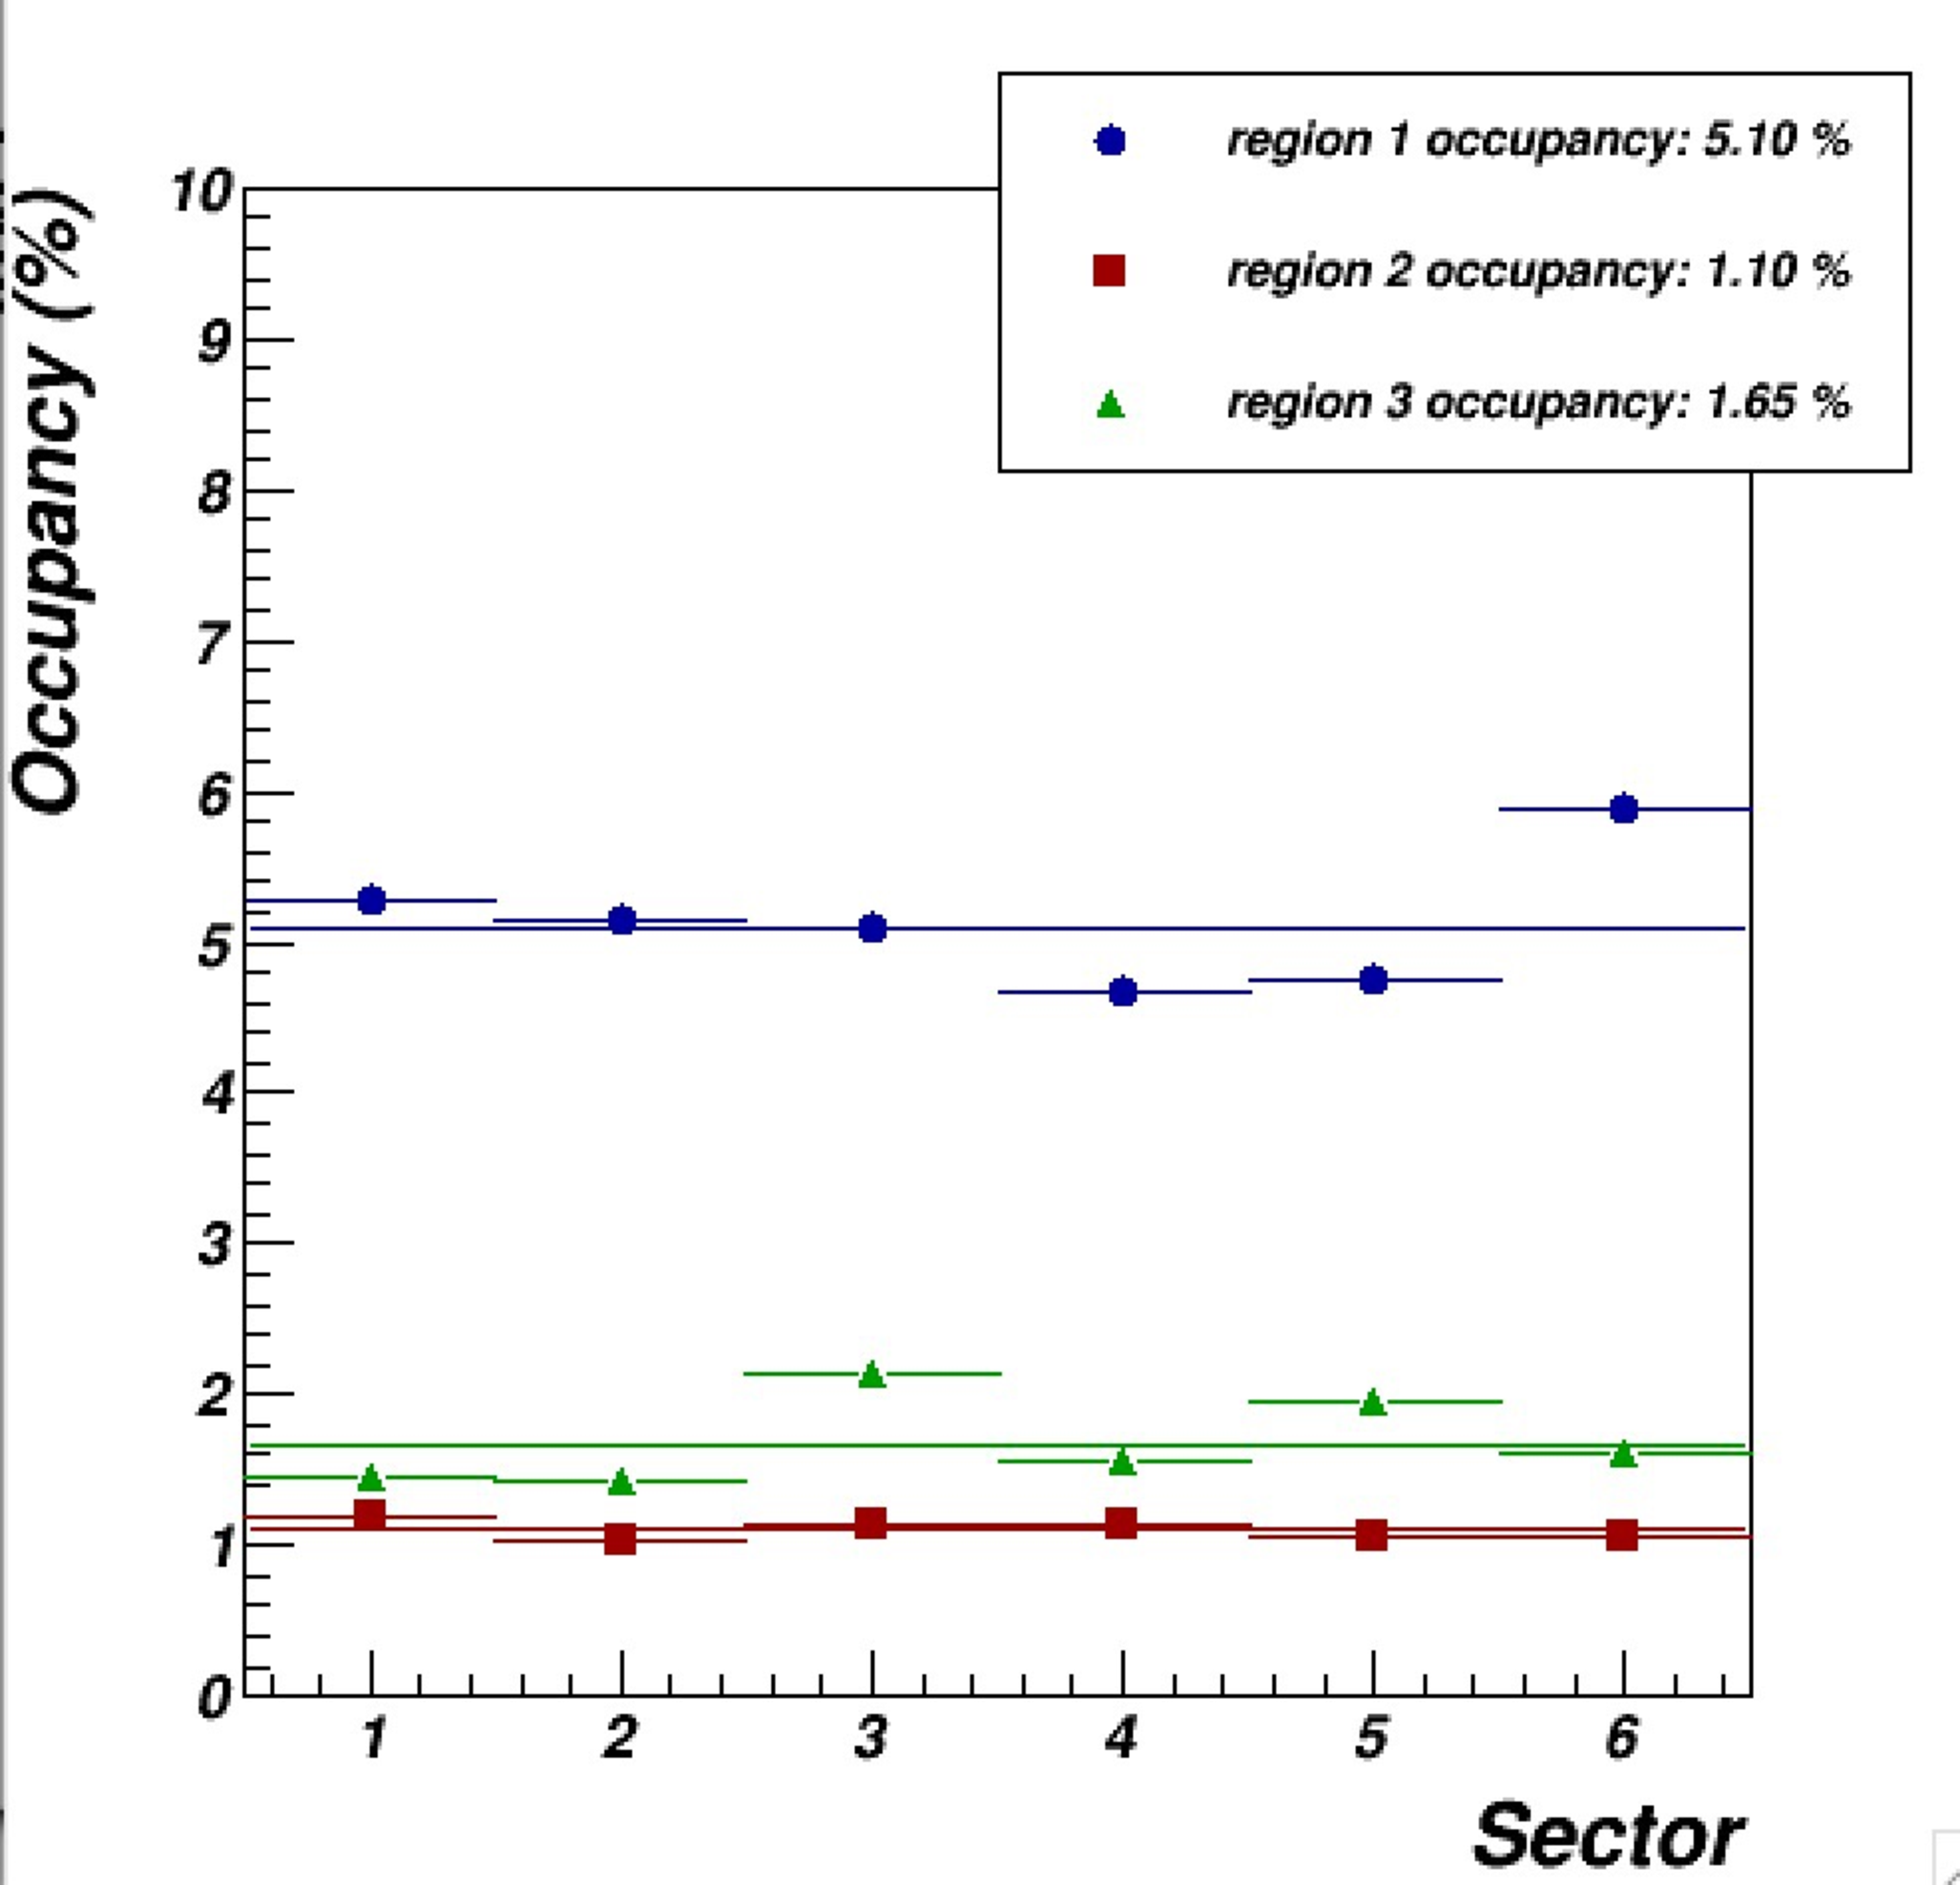
\includegraphics[width=4in]{Angela1.pdf} 
   \caption{DC occupancy, region-by-region, in each sector of CLAS12, for the configuration with FT and a rastered 10-nA beam on an ND$_3$ target.}
   \label{dc_occ}
\end{figure}
In the proposed configuration for this experiment, using this shielding, which is {\bf not yet optimized to be used with a rastered beam}, the DC occupancy is 5\% in region 1 and around 1\% in the other regions. In order to understand if such occupancies are tolerable for the CLAS12 reconstruction, the tracking efficiency was studied comparing the ``with FT'' and ``without FT'' cases (both with raster). This study was performed using GEMC simulations which included background as described in this Subsection, plus electrons generated at fixed kinematics ($p=4$ GeV, $\theta=15^{\circ}$, $\phi=0^{\circ}$). The CLAS12 reconstruction was run over the simulated files, and the tracking efficiency, for both Time-Based Tracking (TBT) and Hit-Based Tracking (HBT), was estimated for the two configurations. Table~\ref{track_eff_table} summarizes the results. 
\begin{table}[htbp]
   \centering
   \begin{tabular}{|c||c||c|} 
	\hline
      Configuration    & HBT efficiency & TBT efficiency \\
	\hline
      FT + raster & 94\% & 85\%\\
      no FT + raster & 91\% & 90\%\\
	\hline
   \end{tabular}
   \caption{Tracking efficiency, estimated analyzing GEMC simulations of single electron plus background, for the two configurations, ``with FT'' and ``without FT'', for 10 nA of beam current.}
   \label{track_eff_table}
\end{table}
An example of a track that is correctly reconstructed in spite of the noise in R1 is shown in Fig.~\ref{tracking_eff}. 
\begin{figure}[htbp] 
   \centering
   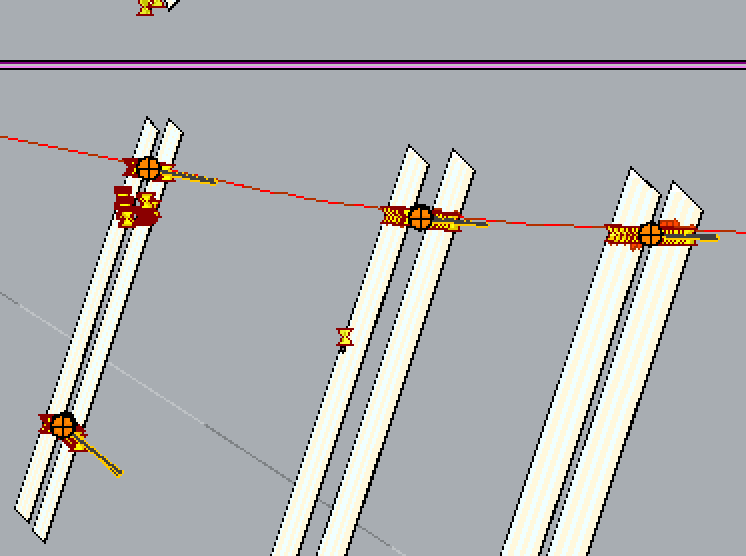
\includegraphics[width=4in]{RecoTrack.png} 
   \caption{Example of one electron track crossing the DCs for the configuration ``with FT - with raster'': the reconstruction works correctly in spite of the noise in R1.}
   \label{tracking_eff}
\end{figure}
There seems to be a 5\% decrease in TBT efficiency between the ``FT'' and ``no FT'' configurations. The higher HBT efficiency for the ``FT'' case could be due to the higher level of fake tracks in region 1. 
It must be pointed out that \cite{veronique_private}:
\begin{itemize}
\item{the shielding for the ``FT'' case is not yet optimized to be used with a rastered beam;}
\item{the tracking code is undergoing development;}
\item{with the current version of the code, the tracking efficiency for non-rastered beam and without any background is 95\%;}
\item{the cuts defining the TBT are not yet adapted to a rastered beam.}
\end{itemize}
The obtained momentum resolution for the 4-GeV electrons is shown in Fig.~\ref{mom_res}: it is 4 MeV, which corresponds to a $dp/p=1$\%, which is equal to the CLAS12 specifications. Thus, the results for the momentum resolution are encouraging. 
\begin{figure}[htbp] 
   \centering
   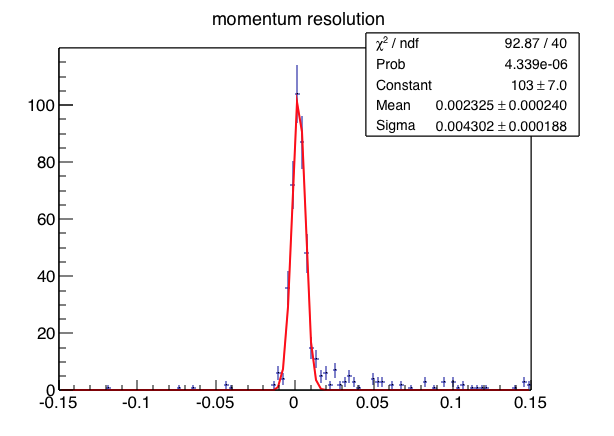
\includegraphics[width=4in]{mom_res_raster.png} 
   \caption{Momentum resolution for simulated 4-GeV electrons, plus background, in the ``with FT'' configuration. }
   \label{mom_res}
\end{figure}
All this considered, it is not fully clear, at the present stage, if a satisfactory tracking efficiency can be obtained when the FT is used and a 10-nA beam is rastered over the ND$_3$ target. %It must also be noted that the EC will also be used for electron identification and measurement of its kinematics. Assuming, as a worse-case scenario, that the current DC tracking efficiency performances were not improved, it could still be possible to use the HBT information coupled to the one from the EC to ensure proper measurement of the electron. 
%and it is not yet clear at this stage what the limit is for the acceptable DC occupancy in CLAS12 to ensure proper tracking, as the tracking reconstruction software is still under development. Preliminary studies \cite{procureur} suggested that tracking should be possible with DC occupancies up to 8-10\%. A definitive answer on this issue can only come when CLAS12 commissioning data will be taken at different beam currents and analyzed with the appropriate tracking and reconstruction software. This proposal is based on the hypothesis that the Forward Tagger can not be used, for the above described reasons. However, if the tracking will prove to be feasible at such levels of DC1 occupancies, the introduction of the Forward Tagger in the setup of this experiment could be beneficial (see Section \ref{sec_countrate} to see the projected asymmetries with and without inclusion of the FT).
\subsection{Radiation dose and backgrounds on the Forward Tagger}
The GEMC simulations containing only the background, for the ``with FT - with raster'' configuration were also used to test the background levels on the Forward Tagger. Figure~\ref{FT_dose} shows the radiation dose (in rad/h) on the crystals of the FT calorimeter. Even in the inner ``rings'', where the backgrounds produced by the beam are at their highest, the dose does not exceed 5 rad/h, which is below the limits of tolerance of the crystals that were selected to be part of the FT \cite{fegan_FT}. 
\begin{figure}[htbp] 
   \centering
   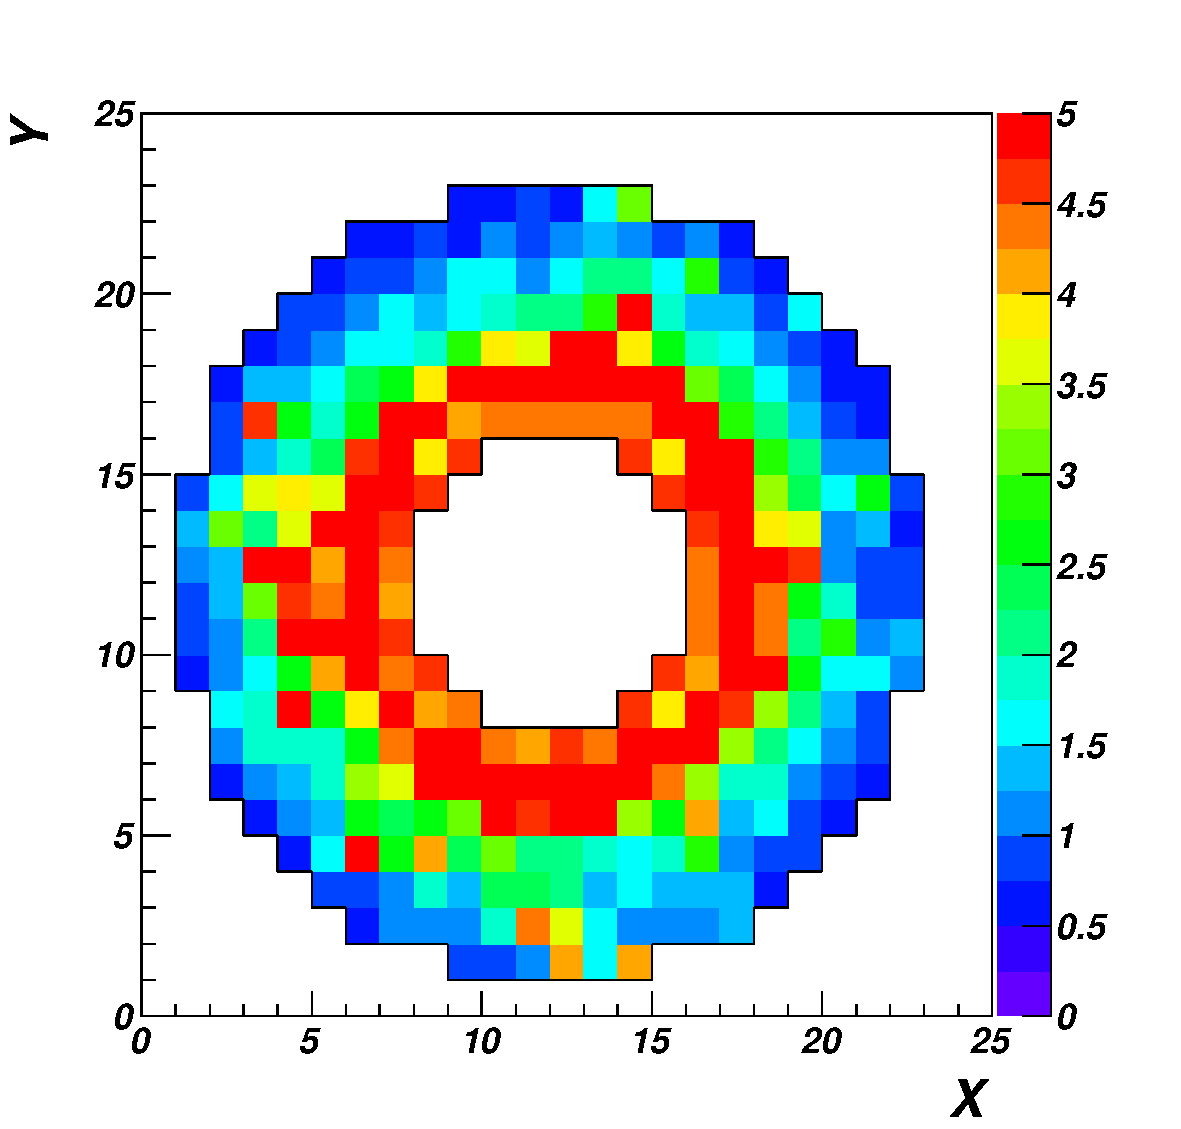
\includegraphics[width=4in]{ft_rad.pdf} 
   \caption{Radiation dose on the FT crystals, obtained from the GEMC background simulations, for the configuration ``with FT - with raster''. The units along $z$ are (rad/h).}
   \label{FT_dose}
\end{figure}
The average energy deposited by the background in the crystals per event was computed integrating over a time window of 120 ns, and it is shown in Fig.~\ref{ft_time}: it is at most around 10 MeV. 
\begin{figure}[htbp] 
   \centering
   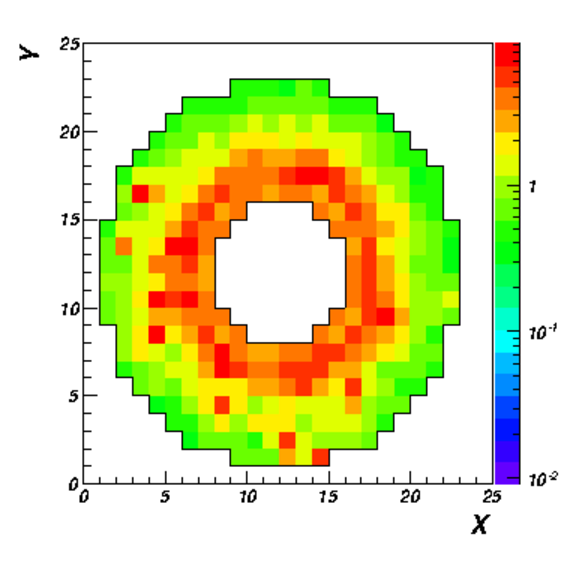
\includegraphics[width=4in]{ft_time.pdf} 
   \caption{Average energy deposit per event in the crystal of the Forward Tagger, obtained with the GEMC background simulations, for the configuration ``with FT - with raster''. The units along $z$ are MeV. }
   \label{ft_time}
\end{figure}
Considering that the typical energies of the photons that will be selected as DVCS candidates are above 2 GeV, the background levels in the FT do not seem critical. 

\subsection{Inclusion of Forward Tagger at 5 nA}
In conclusion, the results of the simulations carried out until now are that if the FT is used with the a 10-nA rastered beam, with the present shielding design, which is not optimized for this setup, and version of the tracking code, the FT itself would not have major problems, but there would be about 5\% of loss in tracking efficiency due to the noise in region 1 of the DC. As the design of the shielding can be further improved for the case in which the beam is rastered, and the tracking algorhytms are also under development, we are hopeful that an optimal configuration will be found that could allow the use of the FT at high luminosity, for the whole duration of the run-group extension. 
However, to be on the safe side, given, on the one hand, the results of the simulations at today, and, on the other hand, the very high cross section that DVCS/BH events have in the kinematics covered by the FT ($\phi\sim 0^{\circ}$ and $\phi\sim 360^{\circ}$), the following plan is adopted for this extension proposal:
\begin{itemize}
\item{run for 50 days at full luminosity (corresponding to 10 nA of beam current) without the Forward Tagger, and}
\item{run for 10 days at half luminosity (5 nA) with the Forward Tagger.}
\end{itemize}
Figure~\ref{dc_occ_5nA} shows the DC occupancies for the FT+raster configuration, with 5 nA of beam current. The value for R1 is low enough to ensure tracking efficiencies above 90\% even with the currently non-optimized version of the reconstruction code. 
\begin{figure}[htbp] 
   \centering
   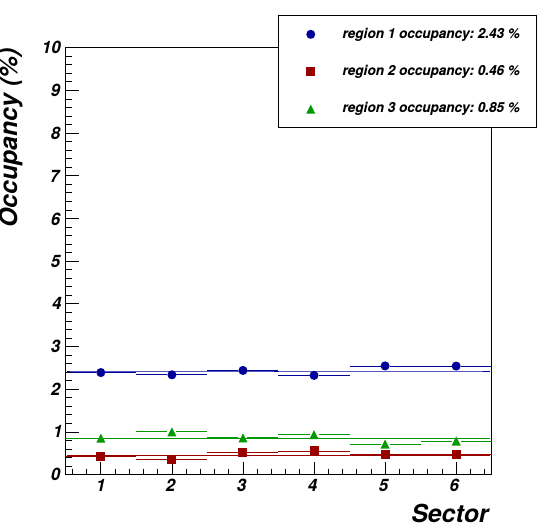
\includegraphics[width=4in]{dc_occ_5nA_FT_detail.png} 
   \caption{DC occupancy, region-by-region, in each sector of CLAS12, for the configuration with FT and a rastered 5-nA beam on an ND$_3$ target.}
   \label{dc_occ_5nA}
\end{figure}
 The following sections will show the expected results for the proposed experiment. 

 
